% ******************************* PhD Thesis Template **************************
% Please have a look at the README.md file for info on how to use the template

\documentclass[a4paper,12pt,fourier,numbered,print,index]{Classes/PhDThesisPSnPDF}

% ******************************************************************************
% ******************************* Class Options ********************************
% *********************** See README for more details **************************
% ******************************************************************************

% `a4paper'(The University of Cambridge PhD thesis guidelines recommends a page
% size a4 - default option) or `a5paper': A5 Paper size is also allowed as per
% the Cambridge University Engineering Deparment guidelines for PhD thesis
%
% `11pt' or `12pt'(default): Font Size 10pt is NOT recommended by the University
% guidelines
%
% `oneside' or `twoside'(default): Printing double side (twoside) or single
% side.
%
% `print': Use `print' for print version with appropriate margins and page
% layout. Leaving the options field blank will activate Online version.
%
% `index': For index at the end of the thesis
%
% `draftclassic': For draft mode without loading any images (same as draft in book)
%
% `draft': Special draft mode with line numbers, images, and water mark with
% timestamp and custom text. Position of the text can also be modified.
%
% `abstract': To generate only the title page and abstract page with
% dissertation title and name, to submit to the Student Registry
%
% `chapter`: This option enables only the specified chapter and it's references
%  Useful for review and corrections.
%
% ************************* Custom Page Margins ********************************
%
% `custommargin`: Use `custommargin' in options to activate custom page margins,
% which can be defined in the preamble.tex. Custom margin will override
% print/online margin setup.
%
% *********************** Choosing the Fonts in Class Options ******************
%
% `times' : Times font with math support. (The Cambridge University guidelines
% recommend using times)
%
% `fourier': Utopia Font with Fourier Math font (Font has to be installed)
%            It's a free font.
%
% `customfont': Use `customfont' option in the document class and load the
% package in the preamble.tex
%
% default or leave empty: `Latin Modern' font will be loaded.
%
% ********************** Choosing the Bibliography style ***********************
%
% `authoryear': For author-year citation eg., Krishna (2013)
%
% `numbered': (Default Option) For numbered and sorted citation e.g., [1,5,2]
%
% `custombib': Define your own bibliography style in the `preamble.tex' file.
%              `\RequirePackage[square, sort, numbers, authoryear]{natbib}'.
%              This can be also used to load biblatex instead of natbib
%              (See Preamble)
%
% **************************** Choosing the Page Style *************************
%
% `default (leave empty)': For Page Numbers in Header (Left Even, Right Odd) and
% Chapter Name in Header (Right Even) and Section Name (Left Odd). Blank Footer.
%
% `PageStyleI': Chapter Name next & Page Number on Even Side (Left Even).
% Section Name & Page Number in Header on Odd Side (Right Odd). Footer is empty.
%
% `PageStyleII': Chapter Name on Even Side (Left Even) in Header. Section Number
% and Section Name in Header on Odd Side (Right Odd). Page numbering in footer

% Uncomment to change page style
%\pagestyle{PageStyleII}

% ********************************** Preamble **********************************
% Preamble: Contains packages and user-defined commands and settings
% ******************************************************************************
% ****************************** Custom Margin *********************************

% Add `custommargin' in the document class options to use this section
% Set {innerside margin / outerside margin / topmargin / bottom margin}  and
% other page dimensions
\ifsetCustomMargin
  \RequirePackage[left=37mm,right=30mm,top=35mm,bottom=30mm]{geometry}
  \setFancyHdr % To apply fancy header after geometry package is loaded
\fi

% Add spaces between paragraphs
%\setlength{\parskip}{0.5em}
% Ragged bottom avoids extra whitespaces between paragraphs
\raggedbottom
% To remove the excess top spacing for enumeration, list and description
%\usepackage{enumitem}
%\setlist[enumerate,itemize,description]{topsep=0em}

% *****************************************************************************
% ******************* Fonts (like different typewriter fonts etc.)*************

% Add `customfont' in the document class option to use this section

\ifsetCustomFont
  % Set your custom font here and use `customfont' in options. Leave empty to
  % load computer modern font (default LaTeX font).
  %\RequirePackage{helvet}

  % For use with XeLaTeX
  %  \setmainfont[
  %    Path              = ./libertine/opentype/,
  %    Extension         = .otf,
  %    UprightFont = LinLibertine_R,
  %    BoldFont = LinLibertine_RZ, % Linux Libertine O Regular Semibold
  %    ItalicFont = LinLibertine_RI,
  %    BoldItalicFont = LinLibertine_RZI, % Linux Libertine O Regular Semibold Italic
  %  ]
  %  {libertine}
  %  % load font from system font
  %  \newfontfamily\libertinesystemfont{Linux Libertine O}
\fi

% *****************************************************************************
% **************************** Custom Packages ********************************

% ************************* Algorithms and Pseudocode **************************

%\usepackage{algpseudocode}


% ********************Captions and Hyperreferencing / URL **********************

% Captions: This makes captions of figures use a boldfaced small font.
%\RequirePackage[small,bf]{caption}

\RequirePackage[labelsep=space,tableposition=top]{caption}
\renewcommand{\figurename}{Fig.} %to support older versions of captions.sty


% *************************** Graphics and figures *****************************

%\usepackage{rotating}
%\usepackage{wrapfig}

% Uncomment the following two lines to force Latex to place the figure.
% Use [H] when including graphics. Note 'H' instead of 'h'
%\usepackage{float}
%\restylefloat{figure}

% Subcaption package is also available in the sty folder you can use that by
% uncommenting the following line
% This is for people stuck with older versions of texlive
%\usepackage{sty/caption/subcaption}
\usepackage{subcaption}

% ********************************** Tables ************************************
\usepackage{booktabs} % For professional looking tables
\usepackage{multirow}

%\usepackage{multicol}
%\usepackage{longtable}
%\usepackage{tabularx}


% *********************************** SI Units *********************************
\usepackage{siunitx} % use this package module for SI units


% ******************************* Line Spacing *********************************

% Choose linespacing as appropriate. Default is one-half line spacing as per the
% University guidelines

% \doublespacing
% \onehalfspacing
% \singlespacing


% ************************ Formatting / Footnote *******************************

% Don't break enumeration (etc.) across pages in an ugly manner (default 10000)
%\clubpenalty=500
%\widowpenalty=500

%\usepackage[perpage]{footmisc} %Range of footnote options


% *****************************************************************************
% *************************** Bibliography  and References ********************

%\usepackage{cleveref} %Referencing without need to explicitly state fig /table

% Add `custombib' in the document class option to use this section
\ifuseCustomBib
   \RequirePackage[square, sort, numbers, authoryear]{natbib} % CustomBib

% If you would like to use biblatex for your reference management, as opposed to the default `natbibpackage` pass the option `custombib` in the document class. Comment out the previous line to make sure you don't load the natbib package. Uncomment the following lines and specify the location of references.bib file

%\RequirePackage[backend=biber, style=numeric-comp, citestyle=numeric, sorting=nty, natbib=true]{biblatex}
%\bibliography{References/references} %Location of references.bib only for biblatex

\fi

% changes the default name `Bibliography` -> `References'
\renewcommand{\bibname}{References}


% ******************************************************************************
% ************************* User Defined Commands ******************************
% ******************************************************************************

% *********** To change the name of Table of Contents / LOF and LOT ************

%\renewcommand{\contentsname}{My Table of Contents}
%\renewcommand{\listfigurename}{My List of Figures}
%\renewcommand{\listtablename}{My List of Tables}


% ********************** TOC depth and numbering depth *************************

\setcounter{secnumdepth}{2}
\setcounter{tocdepth}{2}


% ******************************* Nomenclature *********************************

% To change the name of the Nomenclature section, uncomment the following line

%\renewcommand{\nomname}{Symbols}


% ********************************* Appendix ***********************************

% The default value of both \appendixtocname and \appendixpagename is `Appendices'. These names can all be changed via:

%\renewcommand{\appendixtocname}{List of appendices}
%\renewcommand{\appendixname}{Appndx}

% *********************** Configure Draft Mode **********************************

% Uncomment to disable figures in `draft'
%\setkeys{Gin}{draft=true}  % set draft to false to enable figures in `draft'

% These options are active only during the draft mode
% Default text is "Draft"
%\SetDraftText{DRAFT}

% Default Watermark location is top. Location (top/bottom)
%\SetDraftWMPosition{bottom}

% Draft Version - default is v1.0
%\SetDraftVersion{v1.1}

% Draft Text grayscale value (should be between 0-black and 1-white)
% Default value is 0.75
%\SetDraftGrayScale{0.8}


% ******************************** Todo Notes **********************************
%% Uncomment the following lines to have todonotes.

%\ifsetDraft
%	\usepackage[colorinlistoftodos]{todonotes}
%	\newcommand{\mynote}[1]{\todo[author=kks32,size=\small,inline,color=green!40]{#1}}
%\else
%	\newcommand{\mynote}[1]{}
%	\newcommand{\listoftodos}{}
%\fi

% Example todo: \mynote{Hey! I have a note}

% ************************ Thesis Information & Meta-data **********************
% Thesis title and author information, refernce file for biblatex
% ************************ Thesis Information & Meta-data **********************
%% The title of the thesis
\title{Bayesian Convolutional Neural Network}
%\texorpdfstring is used for PDF metadata. Usage:
%\texorpdfstring{LaTeX_Version}{PDF Version (non-latex)} eg.,
%\texorpdfstring{$sigma$}{sigma}

%% Subtitle (Optional)
%\subtitle{Using the CUED template}

%% The full name of the author
\author{Kumar Shridhar}

%% Department (eg. Department of Engineering, Maths, Physics)
\dept{Department of Computer Science}

%% University and Crest
\university{University of Kaiserslautern}
% Crest minimum should be 30mm.
\crest{
\includegraphics[width=0.2\textwidth]{University_Crest}}
%% Use this crest, if you are using the college crest
%% Crest long miminum should be 65mm
%\crest{
\includegraphics[width=0.45\textwidth]{University_Crest_Long}}

%% College shield [optional] 
% Crest minimum should be 30mm.
%\collegeshield{
\includegraphics[width=0.2\textwidth]{CollegeShields/Kings}}


%% Supervisor (optional)
%% for multiple supervisors, append each supervisor with the \newline command
\supervisor{Prof. Marcus Liwicki\newline
Felix Laumann}

%% Supervisor Role (optional) - Supervisor (default) or advisor
% \supervisorrole{\textbf{Supervisors: }}
%% if no title is desired:
% \supervisorrole{}

%% Supervisor line width: required to align supervisors
\supervisorlinewidth{0.35\textwidth}

%% Advisor (optional)
%% for multiple advisors, append each advisor with the \newline command
%\advisor{Dr. A. Advisor\newline
%Dr. B. Advisor}
     
%% Advisor Role (optional) - Advisor (default) or leave empty
% \advisorrole{Advisors: }
%% if no title is required
% \advisorrole{}

%% Advisor line width: required to align supervisors
%\advisorlinewidth{0.25\textwidth}


%% You can redefine the submission text:
% Default as per the University guidelines:
% ``This thesis is submitted in fulfillment for the degree of''
\renewcommand{\submissiontext}{This thesis is submitted in fulfillment for the degree of}

%% Full title of the Degree
\degreetitle{Master of Science}

%% College affiliation (optional)
%\college{King's College}

%% Submission date
% Default is set as {\monthname[\the\month]\space\the\year}
%\degreedate{September 2014} 

%% Meta information
\subject{Thesis} \keywords{{BayesCNN} {Master Thesis} {Engineering} {University of
Kaiserslautern}}


% ***************************** Abstract Separate ******************************
% To printout only the titlepage and the abstract with the PhD title and the
% author name for submission to the Student Registry, use the `abstract' option in
% the document class.

\ifdefineAbstract
 \pagestyle{empty}
 \includeonly{Declaration/declaration, Abstract/abstract}
\fi

% ***************************** Chapter Mode ***********************************
% The chapter mode allows user to only print particular chapters with references
% Title, Contents, Frontmatter are disabled by default
% Useful option to review a particular chapter or to send it to supervisior.
% To use choose `chapter' option in the document class

\ifdefineChapter
 \includeonly{Chapter3/chapter3}
\fi

% ******************************** Front Matter ********************************
\begin{document}

\frontmatter

\maketitle

%% ******************************* Thesis Dedidcation ********************************

\begin{dedication} 

I would like to dedicate this thesis to the Machine Learning Community \dots

\end{dedication}
% ******************************* Thesis Declaration ***************************

\begin{declaration}

I hereby declare that except where specific reference is made to the work of others, the contents of this thesis are original and have not been submitted in whole or in part for consideration for any other degree or qualification in this, or any other university. This thesis is my own work and contains nothing which is the outcome of work done in collaboration with others, except as specified in the text and in acknowledgements.\\ \\ \\ \\

% Author and date will be inserted automatically from thesis.tex \author \degreedate

\end{declaration}
% ************************** Thesis Acknowledgements **************************

\begin{acknowledgements}      

I would first like to thank my thesis advisor \textbf{Prof. Marcus Liwicki} who was always present physically or virtually whenever I ran into some trouble or had a crazy thought. He consistently steered me in the right the direction whenever he thought I needed it.

I would also like to thank my second thesis advisor \textbf{Felix Laumann} with whom I worked in Copenhagen and in Kaiserslautern. He also made sure Imperial College, London is never far away with our continuous calls and discussion. He assisted in all different work done in the thesis from research to implementation and writing.\\

I would also like to acknowledge \textbf{University of Kaiserlautern} for providing me the opportunity for writing the thesis and \textbf{MindGarage} for providing me the computation power.\\

I must express my very profound gratitude to my parents (\textbf{Vivek} and \textbf{Anita}), to my sister (\textbf{Mineshi}) and to \textbf{Purvanshi Mehta} for providing me with unfailing support and continuous encouragement throughout thesis. 

Finally, I am thankful to \textbf{Ashutosh Mishra}, \textbf{Saurabh Varshneya} and \textbf{Ayushman Dash} for their invaluable comments and endless discussion. I am also thankful to \textbf{Sadique Adnan Siddiqui} for his late night tea and delicious food. This accomplishment would not have been possible without them. \\

I would also like to mention \textbf{BotSupply} for providing me the funds to go and meet new people to discuss ideas. \\ \\



\end{acknowledgements}

% ************************** Thesis Abstract *****************************
% Use `abstract' as an option in the document class to print only the titlepage and the abstract.
\begin{abstract}
Artificial Neural Networks are connectionist systems that learn to perform tasks by learning on examples without having a prior knowledge about the tasks. This is done by finding an optimal point estimate for the weights in every node.
Generally, the network using point estimates as weights perform well with large datasets, but they fail to express uncertainty in regions with little or no data, leading to overconfident decisions.

In this thesis, Bayesian Convolutional Neural Network (BayesCNN) is proposed that introduces probability distribution over the weights. 

BayesCNN is based on Bayes by Backprop which derives a variational approximation to the true posterior. 
Our proposed method not only achieves performances equivalent to frequentist inference in identical architectures but also incorporate a measurement for uncertainties and regularisation. Furthermore, the approach eliminates the use of dropout in the model.

In the first part of the thesis, the Bayesian Neural Network is explained and applied to Image Classification task. The results are compared to point-estimates based architectures on MNIST, CIFAR-10, CIFAR-100 and STL-10 datasets.

In the second part of the thesis, the concept is further applied to other computer vision tasks namely, Image Super-Resolution and Generative Adversarial Networks. The concept of BayesCNN is tested and compared against other concepts in a similar domain.  

\end{abstract}


% *********************** Adding TOC and List of Figures ***********************

\tableofcontents

\listoffigures

\listoftables

% \printnomenclature[space] space can be set as 2em between symbol and description
%\printnomenclature[3em]

\printnomenclature

% ******************************** Main Matter *********************************
\mainmatter

%!TEX root = ../thesis.tex
%*******************************************************************************
%*********************************** First Chapter *****************************
%*******************************************************************************

\chapter{Introduction}  %Title of the First Chapter

\ifpdf
    \graphicspath{{Chapter1/Figs/Raster/}{Chapter1/Figs/PDF/}{Chapter1/Figs/}}
\else
    \graphicspath{{Chapter1/Figs/Vector/}{Chapter1/Figs/}}
\fi


%********************************** %First Section  **************************************

\section{Problem Statement}

Deep Neural Networks (DNNs), are connectionist systems that learn to perform tasks by learning on examples without having a prior knowledge about the tasks. 
They easily scale to millions of data points and yet remain tractable to optimize with stochastic gradient descent.

Convolutional Neural Networks (CNNs), a variant of DNNs, have already surpassed human accuracy in the realm of image classification (e.g. \cite{he2016deep,simonyan2014very,krizhevsky2012imagenet}). Due to the capacity of CNNs to fit on a wide diversity of non-linear data points, they require large amount of training data. This often makes CNNs and Neural Networks in general, prone to overfitting on small datasets. The model tends to fit well to the training data, but are not predictive for new data. This often makes the Neural Networks incapable of correctly assessing the uncertainty in the training data and hence leads to overly confident decisions about the correct class, prediction or action.

Various regularization techniques for controlling overfitting are used in practice namely  early stopping, weight decay, L1, L2 regularizations and currently the most popular and empirically effective technique being \emph{dropout}~\cite{hinton2012improving}. 

We will address both of these concerns by using Bayesian learning to add a measure for uncertainty and regularization in their predictions. 

\section{How to tackle the problem}

Deep Neural Networks have been successfully applied to many domains, including sensitive domains like health-care, security, fraudulent transactions and many more. However, from a probability theory perspective, it is unjustifiable to use single point-estimates as weights to base any classification on.
On the other hand, Bayesian neural networks (NNs) are more robust to over-fittings, and can easily learn from small datasets. Bayesian approach further offers uncertainty estimates via its parameters in form of probability distributions (see Figure \ref{fig:Scalar_Bayesian_Distribution}). At the same time, by using a prior probability distribution to integrate out the parameters, we compute the average across many models during training, which gives a regularization effect to the network, thus preventing overfitting.


Bayesian posterior inference over the neural network parameters is a theoretically attractive method for controlling overfitting; however, modelling a distribution over the kernels (also known as filters) of a CNN has never been attempted successfully before, perhaps because of the vast number of parameters and extremely large models commonly used in practical applications.

Even with a small number of parameters, inferring model posterior in a Bayesian NN is a difficult task. Approximations to the model posterior are often used instead, with variational inference being a popular approach. In this approach one would model the posterior using a simple \textit{variational} distribution such as a Gaussian, and try to fit the distribution's parameters to be as close as possible to the true posterior. This is done by minimising the Kullback-Leibler divergence from the true posterior. Many have followed this approach in the past for standard NN models \citep{hinton1993keeping,barber1998ensemble,graves2011practical,blundell2015weight}.
But the variational approach used to approximate the posterior in Bayesian NNs can be fairly computationally expensive -- the use of Gaussian approximating distributions increases the number of model parameters considerably, without increasing model capacity by much. \citet{blundell2015weight} for example use Gaussian distributions for Bayesian NN posterior approximation and have doubled the number of model parameters, yet report the same predictive performance as traditional approaches using dropout. This makes the approach unsuitable for use with CNNs as the increase in the number of parameters is too costly.

\begin{figure}[t]
\begin{center}
\includegraphics[height=.28\textheight]{Figs/filter_scalars.png}
\includegraphics[height=.28\textheight]{Figs/CNNwithdist.png}
\label{fig:Scalar_Bayesian_Distribution}
\caption{Top: Each filter weight has a fixed value, as in the case of frequentist Convolutional Networks. Bottom: Each filter weight has a distribution, as in case of Bayesian Convolutional Networks.}
\end{center}
\end{figure}

\newline We build our Bayesian \ac{cnn} upon \textit{Bayes by Backprop} \cite{graves2011practical,blundell2015weight}. The exact Bayesian inference on the weights of a neural network is intractable as the number of parameters is very large and the functional form of a neural network does not lend itself to exact integration. So, we approximate the intractable true posterior probability distributions $p(w|\mathcal{D})$ with variational probability distributions $q_{\theta}(w|\mathcal{D})$, which comprise the properties of Gaussian distributions $\mu \in \mathbb{R}^d$ and $\sigma \in \mathbb{R}^d$, denoted $\mathcal{N}(\theta|\mu, \sigma^2)$, where $d$ is the total number of parameters defining a probability distribution. The shape of these Gaussian variational posterior probability distributions, determined by their variance $\sigma^2$, expresses an uncertainty estimation of every model parameter. \\ \\
\newline The main contributions of our work are as follows: 
\begin{enumerate}
    \item We present how \textit{Bayes by Backprop} can be efficiently applied to \acp{cnn}. We therefore introduce the idea of applying two convolutional operations, one for the mean and one for the variance.
    \item We show how the model learn richer representations and predictions from cheap model averaging.
    \item We empirically show that our proposed generic and reliable variational inference method for Bayesian \acp{cnn} can be applied to various \ac{cnn} architectures without any limitations on their performances. 
    \item We examine how to estimate the aleatoric and epistemic uncertainties and empirically show how the uncertainty can decrease, allowing the decisions made by the network to become more deterministic as the training accuracy increases. 
    \item We also empirically show how our method typically only doubles the number of parameters yet trains an infinite ensemble using unbiased Monte Carlo estimates of the gradients. 
\end{enumerate} 
This work builds on the foundations laid out by Blundell et al. \cite{blundell2015weight}, who introduced \textit{Bayes by Backprop} for feedforward neural networks. Together with the extension to recurrent neural networks, introduced by Fortunato et al. \cite{fortunato2017bayesian}, \textit{Bayes by Backprop} is now applicable on the three most frequently used types of neural networks, i.e., feedforward, recurrent, and convolutional neural networks.




\section{Probabilistic Machine Learning} %Section - 1.1 

Lorem Ipsum is simply dummy text of the printing and typesetting industry (see 
Section~\ref{section1.3}). Lorem Ipsum~\citep{Aup91} has been the industry's 
standard dummy text ever since the 1500s, when an unknown printer took a galley 
of type and scrambled it to make a type specimen book. It has survived not only 
five centuries, but also the leap into electronic typesetting, remaining 
essentially unchanged. It was popularised in the 1960s with the release of 
Letraset sheets containing Lorem Ipsum passages, and more recently with desktop 
publishing software like Aldus PageMaker including versions of Lorem 
Ipsum~\citep{AAB95,Con90,LM65}.

The most famous equation in the world: $E^2 = (m_0c^2)^2 + (pc)^2$, which is 
known as the \textbf{energy-mass-momentum} relation as an in-line equation.

A {\em \LaTeX{} class file}\index{\LaTeX{} class file@LaTeX class file} is a file, which holds style information for a particular \LaTeX{}.


\begin{align}
CIF: \hspace*{5mm}F_0^j(a) = \frac{1}{2\pi \iota} \oint_{\gamma} \frac{F_0^j(z)}{z - a} dz
\end{align}

\nomenclature[z-cif]{$CIF$}{Cauchy's Integral Formula}                                % first letter Z is for Acronyms 
\nomenclature[a-F]{$F$}{complex function}                                                   % first letter A is for Roman symbols
\nomenclature[g-p]{$\pi$}{ $\simeq 3.14\ldots$}                                             % first letter G is for Greek Symbols
\nomenclature[g-i]{$\iota$}{unit imaginary number $\sqrt{-1}$}                      % first letter G is for Greek Symbols
\nomenclature[g-g]{$\gamma$}{a simply closed curve on a complex plane}  % first letter G is for Greek Symbols
\nomenclature[x-i]{$\oint_\gamma$}{integration around a curve $\gamma$} % first letter X is for Other Symbols
\nomenclature[r-j]{$j$}{superscript index}                                                       % first letter R is for superscripts
\nomenclature[s-0]{$0$}{subscript index}                                                        % first letter S is for subscripts


%********************************** %Second Section  *************************************

\nomenclature[z-DEM]{DEM}{Discrete Element Method}
\nomenclature[z-FEM]{FEM}{Finite Element Method}
\nomenclature[z-PFEM]{PFEM}{Particle Finite Element Method}
\nomenclature[z-FVM]{FVM}{Finite Volume Method}
\nomenclature[z-BEM]{BEM}{Boundary Element Method}
\nomenclature[z-MPM]{MPM}{Material Point Method}
\nomenclature[z-LBM]{LBM}{Lattice Boltzmann Method}
\nomenclature[z-MRT]{MRT}{Multi-Relaxation 
Time}
\nomenclature[z-RVE]{RVE}{Representative Elemental Volume}
\nomenclature[z-GPU]{GPU}{Graphics Processing Unit}
\nomenclature[z-SH]{SH}{Savage Hutter}
\nomenclature[z-CFD]{CFD}{Computational Fluid Dynamics}
\nomenclature[z-LES]{LES}{Large Eddy Simulation}
\nomenclature[z-FLOP]{FLOP}{Floating Point Operations}
\nomenclature[z-ALU]{ALU}{Arithmetic Logic Unit}
\nomenclature[z-FPU]{FPU}{Floating Point Unit}
\nomenclature[z-SM]{SM}{Streaming Multiprocessors}
\nomenclature[z-PCI]{PCI}{Peripheral Component Interconnect}
\nomenclature[z-CK]{CK}{Carman - Kozeny}
\nomenclature[z-CD]{CD}{Contact Dynamics}
\nomenclature[z-DNS]{DNS}{Direct Numerical Simulation}
\nomenclature[z-EFG]{EFG}{Element-Free Galerkin}
\nomenclature[z-PIC]{PIC}{Particle-in-cell}
\nomenclature[z-USF]{USF}{Update Stress First}
\nomenclature[z-USL]{USL}{Update Stress Last}
\nomenclature[s-crit]{crit}{Critical state}
\nomenclature[z-DKT]{DKT}{Draft Kiss Tumble}
\nomenclature[z-PPC]{PPC}{Particles per cell}

%!TEX root = ../thesis.tex
%*******************************************************************************
%****************************** Second Chapter *********************************
%*******************************************************************************

\newcommand{\ba}{\mathbf{a}}
\newcommand{\bb}{\mathbf{b}}
\newcommand{\bd}{\mathbf{d}}
\newcommand{\bw}{\mathbf{w}}
\newcommand{\bx}{\mathbf{x}}
\newcommand{\by}{\mathbf{y}}
\newcommand{\Exp}[2]{\mathbb{E}_{#1}\left[#2\right]}
\newcommand{\Var}[2]{\text{Var}_{#1}\left[#2\right]}
\newcommand{\Cov}[2]{\text{Cov}_{#1}\left[#2\right]}
\newcommand{\Corr}[2]{\text{Corr}_{#1}\left[#2\right]}

\newcommand{\bA}{\mathbf{A}}
\newcommand{\bB}{\mathbf{B}}
\newcommand{\bV}{\mathbf{V}}
\newcommand{\bW}{\mathbf{W}}
\newcommand{\bv}{\mathbf{v}}

\newcommand{\bphi}{\mathbf{\phi}}
\newcommand{\bt}{\mathbf{\theta}}
\newcommand{\bdelta}{\mathbf{\delta}}
\newcommand{\beps}{\mathbf{\epsilon}}
\newcommand{\q}{q_\mathbf{\phi}}
\newcommand{\bmu}{\mathbf{\mu}}
\newcommand{\bsigma}{\mathbf{\sigma}}
\newcommand{\bSigma}{\mathbf{\Sigma}}

\newcommand{\D}{\mathcal{D}}

\newcommand{\eqnr}{\addtocounter{equation}{1}\tag{\theequation}}

\chapter{Background}

\ifpdf
    \graphicspath{{Chapter2/Figs/Raster/}{Chapter2/Figs/PDF/}{Chapter2/Figs/}}
\else
    \graphicspath{{Chapter2/Figs/Vector/}{Chapter2/Figs/}}
\fi


\fbox{
    \parbox{\textwidth}
    {
       Chapter Overview
        \begin{itemize}
            \item Neural Networks and Convolutional Neural Networks.
            \item Concepts like Variational Inference, and local reparameterization trick in Bayesian Neural Network.
            \item Backpropagation in Bayesian Networks using Bayes by Backprop.
            \item Estimation of Uncertainties in a network.
            \item Pruning a network to reduce the parameters without affecting the performance.
        \end{itemize}
    }
}

\pagebreak

\section{Neural Networks}
\subsection{Brain Analogies}

A perceptron is conceived as a mathematical model of how the neurons function in our brain by a famous psychologist Rosenblatt. According to him, a neuron  takes a set of binary inputs (nearby neurons), multiplies each input by a continuous-valued weight (the synapse strength to each nearby neuron), and thresholds the sum of these weighted inputs to output a 1 if the sum is big enough and otherwise a 0 (in the same way neurons either fire or do not).

\begin{figure}[H]
\begin{center}
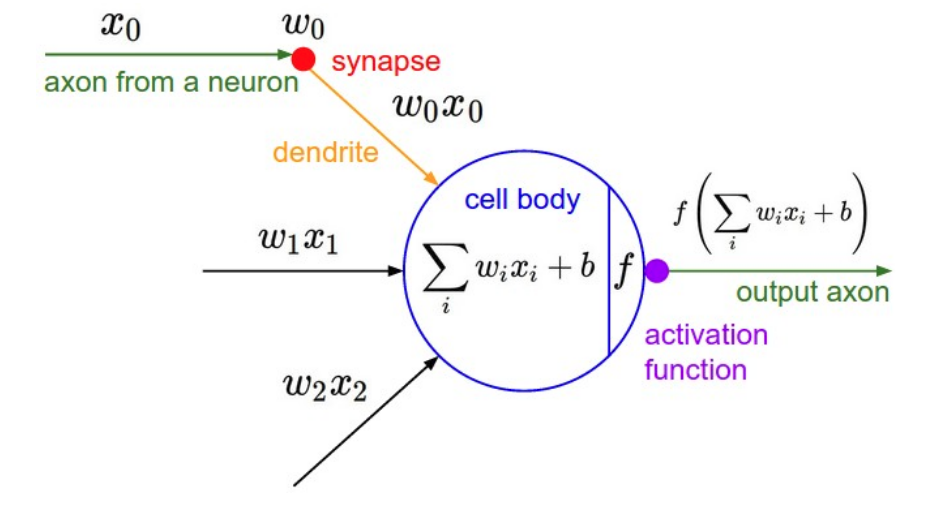
\includegraphics[height=.28\textheight]{Chapter2/Figs/NeuralNetwork.png}
\label{fig:Neural_Network}
\caption{Biologically inspired Neural Network \cite{karparthy}}
\end{center}
\end{figure}

\subsection{Neural Network}

Inspired by the biological nervous system, the structure of an Artificial Neural Network (ANN) is developed to process information similar to how brain process information. A large number of highly interconnected processing elements (neurons) working together makes a Neural Network solve complex problems. Just like humans learn by example, so does a Neural Network. Learning in biological systems involves adjustments to the synaptic connections which is similar to weight updates in a Neural Network. 

A Neural Network consists of three layers: input layer to feed the data to the model to learn representation, hidden layer that learns the representation and the output layer that outputs the results or predictions. Neural Networks can be thought of an end to end system that finds patterns in data which are too complex to be recognized by a human to teach to a machine. 


\begin{figure}[H]
\begin{center}
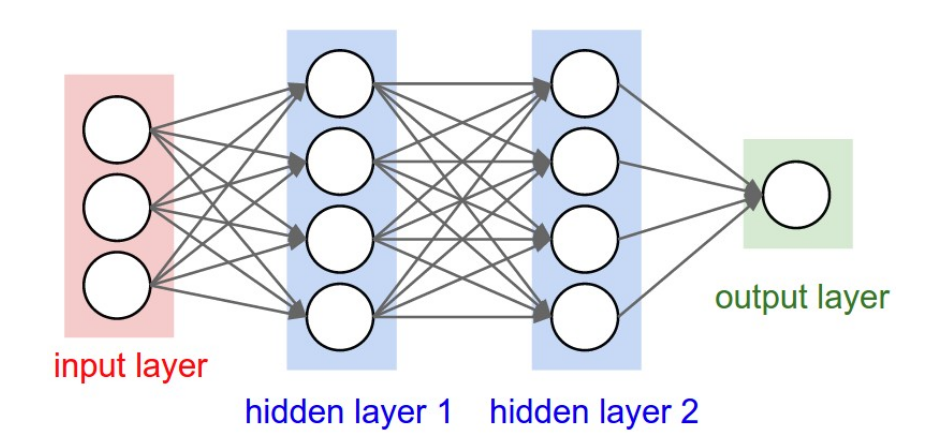
\includegraphics[height=.28\textheight]{Chapter2/Figs/TwoLayeredNN.png}
\label{fig:Two Layered Neural_Network}
\caption{Neural Network with two hidden layers \cite{karparthy}}
\end{center}
\end{figure}


\subsection{Convolutional Neural Network}

Hubel and Wiesel in their hierarchy model mentioned a neural network to have a hierarchy structure in the visual cortex. LGB (lateral geniculate body) forms the simple cells that form the complex cells which form the lower order hypercomplex cells that finally form the higher order hypercomplex cells.
Also, the neural network between lower order hypercomplex cells and higher order hypercomplex cells are structurally similar to the network between simple cells and complex cells. In this hierarchy, a cell in a higher stage generally has a tendency to respond selectively to a more complicated feature of the stimulus pattern, and the cell at the lower stage responds to simpler features. Also, higher stage cells possess a larger receptive field and are more insensitive to the shift in the position of the stimulus pattern.

Similar to a hierarchy model, a neural network starting layers learns simpler features like edges and corners and subsequent layers learn complex features like colours, textures and so on. Unlike in multilayer perceptron where all neurons from one layer are connected with all the neurons in the next layer, weight sharing is the main idea behind a convolutional neural network. 
Example: instead of each neuron having a different weight for each pixel of the input image (28*28 weights), the neurons only have a small set of weights (5x5=25) that is applied a whole bunch of small subsets of the image of the same size. Layers past the first work in a similar way, but take in the ‘local’ features found in the previously hidden layer rather than pixel images, and so ‘see’ successively larger portions of the image since they are combining information about increasingly larger subsets of the image. Finally, the final layer makes the correct prediction for the output class.

The reason for why this is helpful is intuitive if not mathematically clear: without such constraints, the network would have to learn the same simple things (such as detecting edges, corners, etc) a whole bunch of times for each portion of the image. But with the constraint there, only one neuron would need to learn each simple feature - and with far fewer weights overall, it could do so much faster! Moreover, since the pixel-exact locations of such features do not matter the neuron could basically skip neighbouring subsets of the image - subsampling, now known as a type of pooling - when applying the weights, further reducing the training time. The addition of these two types of layers - convolutional and pooling layers - are the primary distinctions of Convolutional Neural Nets (CNNs/ConvNets) from plain old neural nets.


\section{Probabilistic Machine Learning}
\subsection{Variational Inference}

We define a function $y = f(\mathbf{x})$ that estimates the given inputs $\{ x_1, \hdots, x_N \}$ and their corresponding outputs $\{y_1, \hdots, y_N\}$ and produces an output. Using Bayesian inference, a prior distribution is used over the space of functions $p(f)$. This distribution represents our prior belief as to which functions are likely to have generated our data. 

A likelihood is defined as $p(Y | f, X)$ to capture the process in which given a function observation is generated. We use the Bayes rule to find the posterior distribution given our dataset: $p(f | X, Y)$.

The new output can be predicted for a new input point $x^*$ by integrating over all possible functions $f$,
\begin{align} \label{eq:post}
%p(\f | \X, \Y) \propto p(\Y | \X, \f) p(\f).
p(y^* | x^*, X, Y) = \int p(y^* | f^*) p(f^* | x^*, X, Y) df^*
\end{align}

The \eqref{eq:post} is intractable due to the integration sign. We can approximate it by taking a finite set of random variables $w$ and conditioning the model on it. However, it is based on a modelling assumption that the model depends on these variables alone, and making them into sufficient statistics in our approximate model.

The predictive distribution for a new input point $x^*$ is then given by 
$$
p(y^* | x^*, X, Y) = \int p(y^* | f^*) p(f^* | x^*, w) p(w | X, Y) df^* d w.
$$

However, the distribution $p(w | X, Y)$ still remains intractable and we need to approximate it with a variational distribution $q(w)$, that can be computed. The approximate distribution needs to be as close as possible to the posterior distribution obtained from the original model. We thus minimise the Kullback--Leibler (KL) divergence, intuitively a measure of similarity between two distributions: $KL(q(w) ~||~ p(w | X, Y))$,
resulting in the approximate predictive distribution 
\begin{align} \label{eq:predictive}
q(y^* | x^*) = \int p(y^* | f^*) p(f^* | x^*, w) q(w)  df^* dw.
\end{align}

Minimising the Kullback--Leibler divergence is equivalent to maximising the \textit{log evidence lower bound},
\begin{align}
KL_{\text{VI}} := \int q(w) p(F | X, w) \log p(Y | F) dF dw - \KL(q(w) || p(w)) \label{eq:L:VI}
\end{align}
with respect to the variational parameters defining $q(w)$. This is known as \textit{variational inference}, a standard technique in Bayesian modelling.

Maximizing the KL divergence between the posterior and the prior over $w$ will result in a variational distribution that learns a good representation from the data (obtained from log likelihood) and is closer to the prior distribution. In other words, it can prevent overfitting. 


\subsection{Local  reparametrisation  trick}

We therefore propose an alternative estimator for which we have $\Cov{}{L_{i},L_{j}} = 0$, so that the variance of our stochastic gradients scales as $1/M$. We then make this new estimator computationally efficient by not sampling $\beps$ directly, but only sampling the intermediate variables $f(\beps)$ through which $\beps$ influences $L_\D^\text{SGVB}(\bphi)$. By doing so, the global uncertainty in the weights is translated into a form of local uncertainty that is independent across examples and easier to sample. We refer to such a reparameterization from global noise to local noise as the \emph{local reparameterization trick}. Whenever a source of global noise can be translated to local noise in the intermediate states of computation ($\beps \rightarrow f(\beps)$), a local reparameterization can be applied to yield a computationally and statistically efficient gradient estimator.

Such local reparameterization applies to a fairly large family of models but is best explained through a simple example: Consider a standard fully connected neural network containing a hidden layer consisting of 1000 neurons. This layer receives an $M \times 1000$ input feature matrix $\bA$ from the layer below, which is multiplied by a $1000 \times 1000$ weight matrix $\bW$, before a nonlinearity is applied, i.e. $\bB = \bA\bW$. We then specify the posterior approximation on the weights to be a fully factorized Gaussian, i.e.\ $\q(w_{i,j}) = N(\mu_{i,j},\sigma^{2}_{i,j}) \hspace{0.1cm} \forall w_{i,j} \in \bW$, which means the weights are sampled as $w_{i,j} = \mu_{i,j} + \sigma_{i,j}\epsilon_{i,j}$, with $\epsilon_{i,j} \sim N(0,1)$. In this case, we could make sure that $\Cov{}{L_{i},L_{j}} = 0$ by sampling a separate weight matrix $\bW$ for each example in the minibatch, but this is not computationally efficient: we would need to sample $M$ million random numbers for just a single layer of the neural network. Even if this could be done efficiently, the computation following this step would become much harder: Where we originally performed a simple matrix-matrix product of the form $\bB = \bA\bW$, this now turns into $M$ separate local vector-matrix products. The theoretical complexity of this computation is higher, but, more importantly, such a computation can usually not be performed in parallel using fast device-optimized BLAS (Basic Linear Algebra Subprograms). This also happens with other neural network architectures such as convolutional neural networks, where optimized libraries for convolution cannot deal with separate filter matrices per example.

Fortunately, the weights (and therefore $\beps$) only influence the expected log-likelihood through the neuron activations $\bB$, which are of much lower dimension. If we can, therefore, sample the random activations $\bB$ directly, without sampling $\bW$ or $\beps$, we may obtain an efficient Monte Carlo estimator at a much lower cost. For a factorized Gaussian posterior on the weights, the posterior for the activations (conditional on the input $\bA$) is also factorized Gaussian:
\begin{align}
\q(w_{i,j}) &= N(\mu_{i,j},\sigma^{2}_{i,j}) \hspace{0.1cm} \forall w_{i,j} \in \bW \hspace{0.2cm} \Longrightarrow \hspace{0.2cm} \q(b_{m,j}|\bA) = N(\gamma_{m,j},\delta_{m,j}), \text{ with } \nonumber\\
\gamma_{m,j} &= \sum_{i=1}^{1000} a_{m,i}\mu_{i,j}, \hspace{0.2cm} \text{ and } \hspace{0.2cm} \delta_{m,j} = \sum_{i=1}^{1000} a^{2}_{m,i}\sigma^{2}_{i,j}.
\end{align}
Rather than sampling the Gaussian weights and then computing the resulting activations, we may thus sample the activations from their implied Gaussian distribution directly, using $b_{m,j} = \gamma_{m,j} + \sqrt{\delta_{m,j}}\zeta_{m,j}$, with $\zeta_{m,j} \sim N(0,1)$. Here, $\zeta$ is an $M \times 1000$ matrix, so we only need to sample $M$ thousand random variables instead of $M$ million: a thousand fold savings.

In addition to yielding a gradient estimator that is more \textit{computationally efficient} than drawing separate weight matrices for each training example, the local reparameterization trick also leads to an estimator that has \textit{lower variance}. To see why consider the stochastic gradient estimate with respect to the posterior parameter $\sigma^{2}_{i,j}$ for a minibatch of size $M=1$. Drawing random weights $\bW$, we get
\begin{align}
\label{eq:stochest_weights}
\frac{\partial L_\D^\text{SGVB}}{\partial \sigma^{2}_{i,j}} = \frac{\partial L_\D^\text{SGVB}}{\partial b_{m,j}}\frac{\epsilon_{i,j}a_{m,i}}{2\sigma_{i,j}}.
\end{align}
If, on the other hand, we form the same gradient using the local reparameterization trick, we get
\begin{align}
\label{eq:stochest_local}
\frac{\partial L_\D^\text{SGVB}}{\partial \sigma^{2}_{i,j}} = \frac{\partial L_\D^\text{SGVB}}{\partial b_{m,j}}\frac{\zeta_{m,j}a_{m,i}^{2}}{2\sqrt{\delta_{m,j}}}.
\end{align}
Here, there are two stochastic terms: The first is the backpropagated gradient $\partial L_{\D}^\text{SGVB} / \partial b_{m,j}$, and the second is the sampled random noise ($\epsilon_{i,j}$ or $\zeta_{m,j}$). Estimating the gradient with respect to $\sigma^{2}_{i,j}$ then basically comes down to estimating the covariance between these two terms. This is much easier to do for $\zeta_{m,j}$ as there are much fewer of these: individually they have a higher correlation with the backpropagated gradient $\partial L_\D^\text{SGVB}/\partial b_{m,j}$, so the covariance is easier to estimate. In other words, measuring the effect of $\zeta_{m,j}$ on $\partial L_\D^\text{SGVB}/\partial b_{m,j}$ is easy as $\zeta_{m,j}$ is the only random variable directly influencing this gradient via $b_{m,j}$. On the other hand, when sampling random weights, there are a thousand $\epsilon_{i,j}$ influencing each gradient term, so their individual effects get lost in the noise. In appendix \ref{sec:low_variance_reparam} we make this argument more rigorous, and in section~\ref{sec:experiments} we show that it holds experimentally.


%The problem of approximating the gradient thus boils down to estimating one of the correlation coefficients $\rho_{1} = \Corr{q,\D}{\partial L_\D^\text{SGVB}/\partial b_{m,j}, \epsilon_{i,j}}$ or $\rho_{2} = \Corr{q,\D}{\partial L_\D^\text{SGVB}/\partial b_{m,j}, \zeta_{m,j}}$. As is well known, accurately estimating a correlation coefficient is easier if the absolute correlation is large: in general the standard error for the sample correlation coefficient is given by
%\[
%\text{SE}{\rho} = \frac{1 - \rho^{2}}{\sqrt{M - 1}}.
%\]
%Since there are a thousand times fewer $\zeta_{m,j}$ than $\epsilon_{i,j}$, individually they have much higher correlation with the gradient $\partial L_\D^\text{SGVB}/\partial b_{m,j}}$, so they are much easier to estimate. In other words, measuring the effect of $\zeta_{m,j}$ on $\partial L_\D^\text{SGVB}/\partial b_{m,j}}$ is easy as $\zeta_{m,j}$ is the only random variable influencing $b_{m,j}$. On the other hand, when sampling random weights, there are a thousand $\epsilon_{i,j}$ influencing each $b_{m,j}$, so their individual effects get lost in the noise.



%Trivial parallelizability can be retained by translating weight uncertainty in $\q(\bw)$ into local uncertainty in the intermediate states of computation. We call this the \emph{local reparameterisation trick}. Let $\bb^i = f(\ba^i, \bw^i)$ be an intermediate variable of computation for datapoint $i$, with $\ba^i$ a previous state of computation (typically a function of the model input $\bx^i$) and $\bw^i$ the model parameters with distribution $\bw^i \sim \q(\bw)$ that is equal for all $i$. Let $L(\bb^i)$ be (part of) an objective, such as a log-likelihood function, whose expectation w.r.t. $\q(\bw)$ we would like to estimate (equations ~\eqref{eq:bound} and \eqref{eq:objective_sgvb}). Given the distribution $\q(\bw)$, we equivalently have some distribution over $\bb^i$, namely $\q(\bb^i|\ba^i)$. The trick is to parameterize $\bb^i \sim \q(\bb^i|\ba^i)$ as a differentiable function $\bb^i = g^\text{VD}(\beps^i, \ba^i, \bphi)$ with random noise $\beps^i \sim p^\text{VD}(\beps)$, such that:
%\begin{align}
%\Exp{\q(\bw)}{L(f(\ba^i, \bw^i))}
%&= \Exp{\q(\bb^i|\ba^i)}{L(\bb^i)}
%= \Exp{p^\text{VD}(\beps)}{L(g^\text{VD}(\beps^i,\ba^i,\bphi))}
%\end{align}
%The distribution of the original SGVB parameterisation $\bb^i = f(\ba^i, f(\beps^i, \bphi))$ with $\beps^i \sim p(\beps)$, equals the distribution of the new parameterisation $\bb^i = g^\text{VD}(\beps^i, \ba^i, \bphi)$ with $\beps^i \sim p^\text{VD}(\beps)$. The key difference is that computation of $g^\text{VD}(\beps^i, \ba^i, \bphi)$ can often be trivially parallelized, whereas $f(\ba^i, f(\beps^i, \bphi))$ cannot. The resulting operations can be combined into a \emph{variational dropout} (VD) estimator
%\begin{align}
%L_\D(\bphi) \simeq L_\D^\text{VD}(\bphi)
%\label{eq:objective_fsgvb}
%\end{align}
%that is generally much more efficient than $L_\D^\text{SGVB}(\bphi)$ with minibatches.


%\subsection{Fast SGVB through Reparameterization with Local Noise[todo: improve clarity]}\label{sec:fastsgvb}
%
%There is a \emph{de facto} standard strategy for efficiently optimizing objective functions with minibatches of data: vectorize the steps of operations such that the bulk of computation is performed in a small number of large operations, such as large matrix-matrix operations or convolutional operations. Using device-optimized BLAS (Basic Linear Algebra Subprograms) libraries, these few large operations can be automatically and efficiently parallelized across multiple CPU or GPU cores. This strategy is at the heart of efficient implementations in software like Matlab, Theano~\cite{bastien2012theano} and Torch~\cite{collobert2011torch7}, and typically leads to orders of magnitude faster computation than non-vectorized implementations.
%
%A property of $L_\D^\text{SGVB}$ is that the stochasticity is global: weights are sampled from $\q$ only once, then used across all datapoints in the minibatch. This is sub-optimal in terms of variance. A better estimator is one where the noise is independent per datapoint: the variance of the estimator is then inversely proportional to the minibatch size $M$. A first na\"ive attempt is:
%$L_\D^{\text{Na\"ive}}(\bphi) = \frac{N}{M} \sum_{i=1}^M \log p(\by^i|\bx^i,\bw^i)$
%with an explicit separate sample $\bw^i \sim \q(\bw)$ for each individual datapoint $i$ in the minibatch, using a parameterization $\bw^i = f(\beps^i, \bphi)$.
%however, we then lose the ability to easily parallelize this computation, generally leading to drastically slower computation as explained in the previous paragraph. 
%
%[Todo: equation that shows variance reduction effect of separate $\bw^i$ per element in the minibatch.]
%
%Trivial parallelizability can be retained by translating weight uncertainty in $\q(\bw)$ into local uncertainty in the intermediate states of computation. We call this the \emph{local reparameterisation trick}. Let $\bb^i = f(\ba^i, \bw^i)$ be an intermediate variable of computation for datapoint $i$, with $\ba^i$ a previous state of computation (typically a function of the model input $\bx^i$) and $\bw^i$ the model parameters with distribution $\bw^i \sim \q(\bw)$ that is equal for all $i$. Let $L(\bb^i)$ be (part of) an objective, such as a log-likelihood function, whose expectation w.r.t. $\q(\bw)$ we would like to estimate (equations ~\eqref{eq:bound} and \eqref{eq:objective_sgvb}). Given the distribution $\q(\bw)$, we equivalently have some distribution over $\bb^i$, namely $\q(\bb^i|\ba^i)$. The trick is to parameterize $\bb^i \sim \q(\bb^i|\ba^i)$ as a differentiable function $\bb^i = g^\text{local}(\beps^i, \ba^i, \bphi)$ with random noise $\beps^i \sim p^\text{local}(\beps)$, such that:
%\begin{align}
%\Exp{\q(\bw)}{L(f(\ba^i, \bw^i))}
%&= \Exp{\q(\bb^i|\ba^i)}{L(\bb^i)}
%= \Exp{p^\text{local}(\beps)}{L(g^\text{local}(\beps^i,\ba^i,\bphi))}
%\end{align}
%The distribution of the original SGVB parameterisation $\bb^i = f(\ba^i, f(\beps^i, \bphi))$ with $\beps^i \sim p(\beps)$, equals the distribution of the new parameterisation $\bb^i = g^\text{local}(\beps^i, \ba^i, \bphi)$ with $\beps^i \sim p^\text{local}(\beps)$. The key difference is that computation of $g^\text{local}(\beps^i, \ba^i, \bphi)$ can often be trivially parallelized, whereas $f(\ba^i, f(\beps^i, \bphi))$ cannot. The resulting operations can be combined into a \emph{fast SGVB} estimator
%\begin{align}
%L_\D(\bphi) \simeq L_\D^\text{F-SGVB}(\bphi)
%\label{eq:objective_fsgvb}
%\end{align}
%that is generally much more efficient than $L_\D^\text{SGVB}(\bphi)$ with minibatches.

%\subsection{Example: Dot Product, Gaussian Weight Uncertainty}
%Let us give an example of the local reparameterization trick, with the common linear operation $\bb^i = \ba^i \bW$, where the row vector $\ba^i$ is of dimension $1 \times N_A$ and is the result of earlier operations, and $\bb^i$ is of dimension $1 \times N_B$. Let $\bW$ be a parameter matrix, with approximate posterior $\q(\bW) = \prod_{jk}\q(W_{jk})$, with $\q(W_{jk}) = \mathcal{N}(\mu_{jk},\bSigma_{jk})$ where $\bmu$ and $\bSigma$ are variational parameter matrices. With $(\odot, (.)^2, \sqrt{(.)})$ we denote element-wise product, square and square-root.
%
%A non-parallelizable parameterisation of $\bb^i$, is: $\bb^i = \ba^i (\bmu+\beps^i \odot \sqrt{\bSigma})$.
%
%A trivially parallelizable reparameterisation of $\bb^i$ with local noise $\epsilon^i \sim \mathcal{N}(0,I)$ is: $\bb^i = \ba^i \bmu + \epsilon^i \odot \sqrt{(\ba^i)^2 \bSigma}$. Let $\bB = \bA \bW$, where $\bA$ is a matrix of size $M \times N_A$ with $\ba^i$ as $i$-th row, and $\bB$ is the corresponding result with size $M \times N_B$. The vectorized form is $\bB = \bA \bmu + \epsilon \odot \sqrt{\bA^2 \bSigma}$. In this form, most of the computation is contained in a few large matrix-matrix operations, whose computation is trivially parallelized.


\section{Weight Uncertainities}
\subsection{Bayesian Uncertainities}

Uncertainties in a network is a measure of how certain the model is with its prediction. In Bayesian modeling, there are two main types of uncertainty one can model \citep{der2009aleatory}: \textit{Aleatoric} uncertainty and \textit{Epistemic} uncertainty on. 

\textit{Aleatoric} uncertainty measures the noise inherent in the observations. This type of uncertainty is present in the data collection method like the sensor noise or motion noise which is uniform along the dataset. This cannot be reduced if more data is collected. \textit{Epistemic} uncertainty, on the other hand, represents the uncertainty in the model. This uncertainty can be reduced given more data and is often referred to as \textit{model uncertainty}.  Aleatoric uncertainty can further be categorized into \textit{homoscedastic} uncertainty, uncertainty which stays constant for different inputs, and \textit{heteroscedastic} uncertainty. Heteroscedastic uncertainty depends on the inputs to the model, with some inputs potentially having more noisy outputs than others. Heteroscedastic uncertainty is in particular important so that model prevents from outputting very confident decisions.

Existing uncertainties are calculated by placing a probability distributions over either the model parameters or model outputs. Epistemic uncertainty is modelled by placing a prior distribution over a model's weights and then trying to capture how much these weights vary given some data. Aleatoric uncertainty, on the other hand, is modelled by placing a distribution over the output of the model.

\subsubsection{Sources of Uncertainities}

The following can be the source of uncertainty as mentioned by Kiureghian \cite{Kiureghian}:

\begin{enumerate}
    \item Uncertainty inherent in the basic random variables $X$, such as the uncertainty inherent in material property constants and load values, which can be directly measured.
    \item Uncertain model error resulting from the selection of the form of the probabilistic sub-model $f_{X}(x,H_{f})$ used to describe the distribution of basic variables.
    \item  Uncertain modeling errors resulting from selection of the physical sub-models $g_{i}(x,H_{g}), i = 1,2,...,m,$ used to describe the derived variables.
    \item  Statistical uncertainty in the estimation of the parameters $H_f$ of the probabilistic sub-model.
    \item  Statistical uncertainty in the estimation of the parameters $H_g$ of the physical sub-models.
    \item  Uncertain errors involved in measuring of observations, based on which the parameters $H_f$ and $H_g$  are estimated. These include errors involved in indirect measurement, e.g., the measurement of a quantity through a proxy, as in non-destructive testing of material strength.
    \item Uncertainty modelled by the random variables $Y$ corresponding to the derived variables $y$, which may include, in addition to all the above uncertainties, uncertain errors resulting from computational errors, numerical approximations or truncations. For example, the computation of load effects in a nonlinear structure by a finite element procedure employs iterative calculations, which invariably involve convergence tolerances and truncation errors.
\end{enumerate} 

\section{Backpropagation}

Backpropagation is a Neural Networks was proposed by Rumelhart \cite{Rumelhart} in 1986 and it is the most commonly used method for training neural networks. Backpropagation is a technique to compute the gradient of the loss in terms of the network weights. It operates in two phase: firstly, the input features through the network propagates in the forward direction to compute the function output and thereby the loss associated with the parameters. Secondly, the derivatives of the training loss with respect to the weights
are propagated back from the output layer towards the input layers.
These computed derivatives are further used to update the weights of the network. This is a continuous process and updating of the weight occurs continuously over every iteration. 

Despite the popularity of backpropagation, there are many hyperparameters in backpropagation based stochastic optimization that requires specific tuning, e.g., learning rate, momentum, weight decay, etc. The time required for finding the optimal values is proportional to the data size. For a network trained with backpropagation, only point estimates of the weights are achieved in the network. As a result, these networks make overconfident predictions and do not account for uncertainty in the parameters. Lack of uncertainty measure makes the network prone to overfitting and a need for regularization.

A Bayesian approach to Neural Networks provides the shortcomings with the backpropagation approach \cite{mackay1996hyperparameters} as Bayesian methods naturally account for uncertainty in parameter estimates and can propagate this uncertainty into predictions.
Also, averaging over parameter values instead of just choosing single point estimates makes the model robust to overfitting. 

Sevreal approaches has been proposed in the past for learning in Bayesian Networks: Laplace approximation \cite{Mackay1991APB}, MC Dropout \cite{gal2015bayesian},and Variational Inference \cite{hinton1993keeping} \cite{graves2011practical} \cite{blundell2015weight}. We used Bayes by Backprop \cite{blundell2015weight} for our work and is explained next.

\subsection{Bayes by Backprop}
\textit{Bayes by Backprop} \cite{graves2011practical, blundell2015weight} is a variational inference method to learn the posterior distribution on the weights $w \sim q_{\theta}(w|\mathcal{D})$ of a neural network from which weights $w$ can be sampled in backpropagation. 
It regularises the weights by minimising a compression cost, known as the variational free energy or the expected lower bound on the marginal likelihood.

Since the true posterior is typically intractable, an approximate distribution $q_{\theta}(w|\mathcal{D})$ is defined that is aimed to be as similar as possible to the true posterior $p(w|\mathcal{D})$, measured by the Kullback-Leibler (KL) divergence \cite{kullback1951information}. Hence, we define the optimal parameters $\theta^{opt}$ as
\begin{equation}
    \begin{aligned} \label{KL}
        \theta^{opt}&=\underset{\theta}{\text{arg min}}\ \text{KL} \ [q_{\theta}(w|\mathcal{D})\|p(w|\mathcal{D})] \\
        &=\underset{\theta}{\text{arg min}}\ \text{KL} \ [q_{\theta}(w|\mathcal{D})\|p(w)] \\ & -\mathbb{E}_{q(w|\theta)}[\log p(\mathcal{D}|w)]+\log p(\mathcal{D})
    \end{aligned}
\end{equation}

where
\begin{equation}
    \text{KL} \ [q_{\theta}(w|\mathcal{D})\|p(w)]= \int q_{\theta}(w|\mathcal{D})\log\frac{q_{\theta}(w|\mathcal{D})}{p(w)}dw .
\end{equation}
This derivation forms an optimisation problem with a resulting cost function widely known as \textit{variational free energy} \cite{neal1998view,yedidia2005constructing,friston2007variational} which is built upon two terms: the former, $\text{KL} \ [q_{\theta}(w|\mathcal{D})\|p(w)]$, is dependent on the definition of the prior $p(w)$, thus called complexity cost, whereas the latter, $\mathbb{E}_{q(w|\theta)}[\log p(\mathcal{D}|w)]$, is dependent on the data $p(\mathcal{D}|w)$, thus called likelihood cost. 
The term $\log p(\mathcal{D})$ can be omitted in the optimisation because it is constant.
\newline Since the KL-divergence is also intractable to compute exactly, we follow a stochastic variational method \cite{graves2011practical,blundell2015weight}.
We sample the weights $w$ from the variational distribution $q_{\theta}(w|\mathcal{D})$ since it is much more probable to draw samples which are appropriate for numerical methods from the variational posterior $q_{\theta}(w|\mathcal{D})$ than from the true posterior $p(w|\mathcal{D})$. Consequently, we arrive at the tractable cost function \eqref{cost} which is aimed to be optimized, i.e. minimised w.r.t. $\theta$, during training:
\begin{equation} \label{cost}
    \mathcal{F}(\mathcal{D}, \theta)\approx \sum_{i=1}^n \log q_{\theta}(w^{(i)}|\mathcal{D})-\log p(w^{(i)})-\log p(\mathcal{D}|w^{(i)})
\end{equation}
%
where $n$ is the number of draws.
\newline We sample $w^{(i)}$ from $q_{\theta}(w|\mathcal{D})$. The uncertainty afforded by \textit{Bayes by Backprop} trained neural networks has been used successfully for training feedforward neural networks in both supervised and reinforcement learning environments \cite{blundell2015weight,lipton2016efficient,houthooft2016curiosity}, for training recurrent neural networks \cite{fortunato2017bayesian}, but has not been applied to convolutional neural networks to-date.

\section{Model weights pruning}

Model pruning reduces the sparsity in a deep neural network's
various connection matrices, thereby reducing the number of valued parameters in the model. The whole idea of model pruning is to reduce the number of parameters without much loss in the accuracy of the model. This reduces the use of a large parameterized model with regularization and promotes the use of dense connected smaller models. Some recent work suggests \cite{DBLP:journals/corr/HanMD15} \cite{DBLP:journals/corr/NarangDSE17} showed in their work that the network can achieve a sizable reduction in model size, yet achieving comparable accuracy. 
Model pruning possesses several advantages in terms of reduction in computational cost, inference time and in energy-efficiency. The resulting pruned model typically has sparse connection matrices, so
efficient inference using these sparse models requires purpose-built hardware capable of loading sparse matrices and/or performing sparse matrix-vector operations. Thus the overall memory usage is reduced with the new pruned model. 


There are several ways of achieving the pruned model, the most popular one is to map the low contributing weights to zero and reducing the number of overall non-zero valued weights. This can be achieved by training a large sparse model and pruning it further which makes it comparable to training a small dense model. Pruning away the less salient features to zero has been used in this thesis and is explained in details in chapter 4. 



%!TEX root = ../thesis.tex
%*******************************************************************************
%****************************** Third Chapter **********************************
%*******************************************************************************
\chapter{Related Work}

% **************************** Define Graphics Path **************************
\ifpdf
    \graphicspath{{Chapter3/Figs/Raster/}{Chapter3/Figs/PDF/}{Chapter3/Figs/}}
\else
    \graphicspath{{Chapter3/Figs/Vector/}{Chapter3/Figs/}}
\fi

\fbox{
    \parbox{\textwidth}
    {
        Chapter Overview
        \begin{itemize}
            \item How Bayesian Methods were applied to Neural Networks for the intractable true posterior distribution.
            \item Various ways of training Neural Networks posterior probability distributions : Laplace approximations, Monte Carlo and Variational Inference.
            \item Proposals on Dropout and Gaussian Dropout as Variational Inference schemes.
            \item Work done in the past for uncertainity estimation in Neural Network.
            \item Ways to reduce the number of parameters in a model.
        \end{itemize}
    }
}

\pagebreak

\section{Related Work}

\subsection{Bayesian training}
Applying Bayesian methods to neural networks has been studied in the past with various approximation methods for the intractable true posterior probability distribution $p(w|\mathcal{D})$. Buntine and Weigend \cite{buntine1991bayesian} started to propose various \textit{maximum-a-posteriori} (MAP) schemes for neural networks. They were also the first who suggested second order derivatives in the prior probability distribution $p(w)$ to encourage smoothness of the resulting approximate posterior probability distribution.
In subsequent work by Hinton and Van Camp \cite{hinton1993keeping}, the first variational methods were proposed which naturally served as a regularizer in neural networks. He also mentioned that the amount of information in a weight can be controlled by adding Gaussian noise. When optimizing the trade off between the expected error and the information in the weights, the noise level can be adapted during learning.


Hochreiter and Schmidhuber \cite{hochreiter1995simplifying} suggested taking an information theory perspective into account and utilising a minimum description length (MDL) loss. This penalises non-robust weights by means of an approximate penalty based upon perturbations of the weights on the outputs.
Denker and LeCun \cite{denker1991transforming}, and MacKay \cite{mackay1995probable} investigated the posterior probability distributions of neural networks and treated the search in the model space (the space of architectures, weight decay, regularizers, etc..) as an inference problem and tried to solve it using Laplace approximations.
As a response to the limitations of Laplace approximations, Neal \cite{neal2012bayesian} investigated the use of hybrid Monte Carlo for training neural networks, although it has so far been difficult to apply these to the large sizes of neural networks built in modern applications. 
However,these approaches lacked scalability in terms of both the network architecture and the data size. 


More recently, Graves \cite{graves2011practical} derived a variational inference scheme for neural networks and Blundell et al. \cite{blundell2015weight} extended this with an update for the variance that is unbiased and simpler to compute. Graves \cite{graves2016stochastic} derives a similar algorithm in the case of a mixture posterior probability distribution. 
A more scalable solution based on expectation propagation was proposed by Soudry \cite{Soudry:NIPS2014_5269} in 2014. While this method works for networks with binary weights, its extension to continuous weights is unsatisfying as it does not produce estimates of posterior variance.

\newline Several authors have claimed that Dropout \cite{srivastava2014dropout} and Gaussian Dropout \cite{wang2013fast} can be viewed as approximate variational inference schemes \cite{gal2015bayesian, kingma2015variational}. We compare our results to Gal's \& Ghahramani's \cite{gal2015bayesian} and discuss the methodological differences in detail.


\subsection{Uncertainties estimation}

Neural Networks can predict uncertainty when Bayesian methods are introduced in it. An attempt to model uncertainty has been studied from 1990's \cite{neal2012bayesian} but has not been applied successfully until 2015. Gal and Gharmani \cite{Gal2015Dropout} in 2015 provided a theoretical framework for modeling Bayesian uncertainty. Gal and Gharmani \cite{gal2015bayesian} obtained the uncertainty estimates by casting dropout training in conventional deep networks as a Bayesian approximation of a Gaussian Process. They showed that any network trained with dropout is an approximate Bayesian model, and uncertainty estimates can be obtained by computing the variance on multiple predictions with different dropout masks.

\subsection{Model Pruning}

Some early work in the model pruning domaoin used a second-order Taylor approximation of the increase in the loss function of the network when a weight is set to zero \cite{lecun1990optimal}. A diagonal Hessian approximation was used to calculate the saliency for each parameter \cite{lecun1990optimal} and the low-saliency parameters were pruned from the network and the network was retrained.


Narang \cite{DBLP:journals/corr/NarangDSE17} showed that a pruned RNN and GRU model performed better for the task of speech recognition compared to a dense network of original size. This result is very similar to the results obtained in our case where a pruned model achieved better results than a normal network. However, no comparisons can be drawn as the model architecture (CNN vs RNN) used and the tasks (Computer Vision vs Speech Recogniton) are completely different.  Narang \cite{DBLP:journals/corr/NarangDSE17} in his work introduced a gradual pruning scheme based on pruning all the weights in a layer
less than some threshold (manually chosen) which is linear with some
slope in phase 1 and linear with some slope in phase 2 followed by
normal training. However, we reduced the number of filters to half for one case and in the other case, we induced a sparsity based on L1 regularization to remove the less contributing weights and reduced the parameters. 


Other similar work \cite{DBLP:journals/corr/AnwarHS15, DBLP:journals/corr/LebedevGROL14, DBLP:journals/corr/ChangpinyoSZ17} to our work that reduces or removed the redundant connections or induces sparsity are motivated by the desire to speed up computation.
The techniques used are highly convolutional layer dependent and is not applicable to other architectures like Recurrent Neural Networks. 
One another interesting method of pruning is to represent each parameter with a smaller floating point number like 16-bits instead of 64 bits. This way there is a speed up in the training and inference speed and the model is less computationally expensive. 

Another different viewpoint for model compression was presented by Gong \cite{DBLP:journals/corr/GongLYB14}. He proposed vector quantization to achieve different compression ratios and different accuracies and depending on the use case, the compression and accuracies can be choosed. However, it requires a different hardware architecture to support the inference at runtime. Besides quantization, other potentially complementary approaches to reducing model size include low-rank matrix factorization \cite{denton2014exploiting, DBLP:journals/corr/LebedevGROL14} and group sparsity regularization to arrive at an optimal layer size \cite{DBLP:conf/nips/AlvarezS16}.



%!TEX root = ../thesis.tex
%*******************************************************************************
%****************************** Second Chapter *********************************
%*******************************************************************************

\chapter{Concept}

\ifpdf
    \graphicspath{{Chapter2/Figs/Raster/}{Chapter2/Figs/PDF/}{Chapter2/Figs/}}
\else
    \graphicspath{{Chapter2/Figs/Vector/}{Chapter2/Figs/}}
\fi

\fbox{
    \parbox{\textwidth}
    {
        Chapter Overview
        \begin{itemize}
            \item Bayesian \acp{cnn} with Variational Inference based on Bayes by Backprop.
            \item Bayesian convolutional operations with mean and variance
            \item Local reparameterization trick for Bayesian \acp{cnn}.
            \item Uncertainty estimation in a Bayesian network.
            \item Using L1 norm for reducing the number of parameters in a Bayesian network.
        \end{itemize}
    }
}

\pagebreak

\section{Bayesian convolutional neural networks with variational inference}
In this section, we explain our algorithm of building a \ac{cnn} with probability distributions over its weights in each filter, as seen in Figure \ref{fig:filter_scalar}, and apply variational inference, i.e. \textit{Bayes by Backprop}, to compute the intractable true posterior probability distribution, as described in the last Chapter. Notably, a fully Bayesian perspective on a \ac{cnn} is for most \ac{cnn} architectures not accomplished by merely placing probability distributions over weights in convolutional layers; it also requires probability distributions over weights in fully-connected layers (see Figure \ref{fig:CNNwithdist_grey}). 
%
\begin{figure}[H] 
\centering
\begin{minipage}{.4\textwidth}
\centering
\includegraphics[width=\linewidth]{Chapter4/Figs/filter_scalars.png}
\end{minipage}
%
\begin{minipage}{.4\textwidth}
\centering
\includegraphics[width=\linewidth]{Chapter4/Figs/CNNwithdist.png}
\end{minipage}
\caption{Input image with exemplary pixel values, filters, and corresponding output with point-estimates (top) and probability distributions (bottom) over weights.}
\label{fig:filter_scalar}
\end{figure} 
%
\begin{figure}[b!] 
\begin{center}
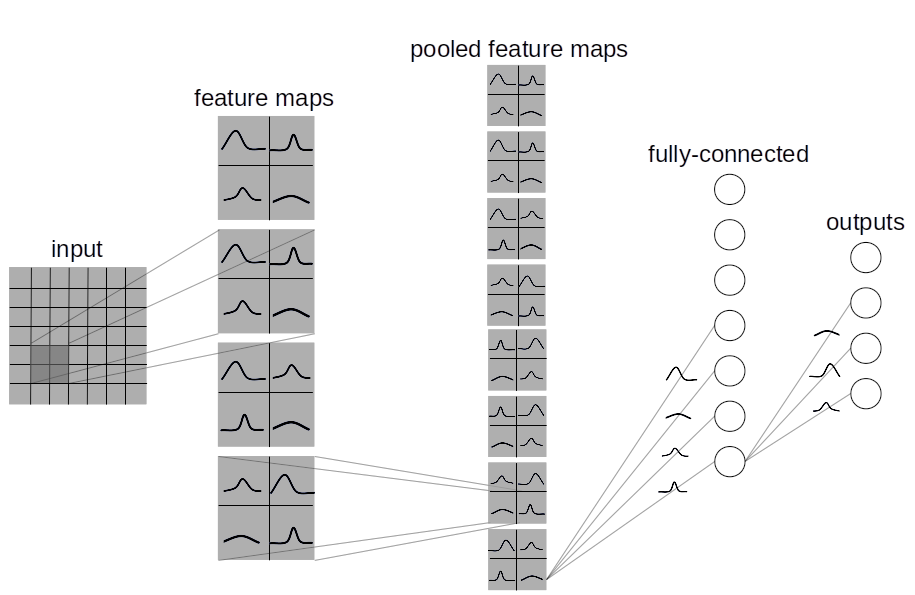
\includegraphics[width=\linewidth]{Chapter4/Figs/CNNwithdist_grey.png}
\caption{Fully Bayesian perspective of an exemplary CNN. Weights in filters of convolutional layers, and weights in fully-connected layers have the form of a probability distribution.}
\label{fig:CNNwithdist_grey}
\end{center}
\end{figure} 
%
\subsection{Local reparameterization trick for convolutional layers}
We utilise the local reparameterization trick \cite{kingma2015variational} and apply it to \acp{cnn}. Following \cite{kingma2015variational,neklyudov2018variance}, we do not sample the weights $w$, but we sample instead layer activations $b$ due to its consequent computational acceleration. The variational posterior probability distribution $q_{\theta}(w_{ijhw}|\mathcal{D})=\mathcal{N}(\mu_{ijhw},\alpha_{ijhw}\mu^2_{ijhw})$ (where $i$ and $j$ are the input, respectively output layers, $h$ and $w$ the height, respectively width of any given filter) allows to implement the local reparamerization trick in convolutional layers. This results in the subsequent equation for convolutional layer activations $b$:
\begin{equation}
    b_j=A_i\ast \mu_i+\epsilon_j\odot \sqrt{A^2_i\ast (\alpha_i\odot \mu^2_i)}
\end{equation}
where $\epsilon_j \sim \mathcal{N}(0,1)$, $A_i$ is the receptive field, $\ast$ signalises the convolutional operation, and $\odot$ the component-wise multiplication.

\subsection{Applying two sequential convolutional operations (mean and variance)}
The crux of equipping a \ac{cnn} with probability distributions over weights instead of single point-estimates and being able to update the variational posterior probability distribution $q_{\theta}(w|\mathcal{D})$ by backpropagation lies in applying \textit{two} convolutional operations whereas filters with single point-estimates apply \textit{one}. As explained in the last chapter, we deploy the local reparametrization trick and sample from the output $b$. Since the output $b$ is a function of mean $\mu_{ijwh}$ and variance $\alpha_{ijhw}\mu^2_{ijhw}$ among others, we are then able to compute the two variables determining a Gaussian probability distribution, namely mean $\mu_{ijhw}$ and variance $\alpha_{ijhw}\mu^2_{ijhw}$, separately. 
\newline We do this in two convolutional operations: in the first, we treat the output $b$ as an output of a \ac{cnn} updated by frequentist inference. We optimize with Adam \cite{kingma2014adam} towards a single point-estimate which makes the validation accuracy of classifications increasing. We interpret this single point-estimate as the mean $\mu_{ijwh}$ of the variational posterior probability distributions $q_{\theta}(w|\mathcal{D})$. In the second convolutional operation, we learn the variance $\alpha_{ijhw}\mu^2_{ijhw}$. As this formulation of the variance includes the mean $\mu_{ijwh}$, only $\alpha_{ijhw}$ needs to be learned in the second convolutional operation \cite{molchanov2017variational}. In this way, we ensure that only one parameter is updated per convolutional operation, exactly how it would have been with a \ac{cnn} updated by frequentist inference. 
\newline In other words, while we learn in the first convolutional operation the MAP of the variational posterior probability distribution $q_{\theta}(w|\mathcal{D})$, we observe in the second convolutional operation how much values for weights $w$ deviate from this MAP. This procedure is repeated in the fully-connected layers. In addition, to accelerate computation, to ensure a positive non-zero variance $\alpha_{ijhw}\mu^2_{ijhw}$, and to enhance accuracy, we learn $\log \alpha_{ijhw}$ and use the \textit{Softplus} activation function as further described in the Experiments section.
%
\section{Uncertainty estimation in CNN}
In classification tasks, we are interested in the predictive distribution $p_{\mathcal{D}}(y^*|x^*)$, where $x^*$ is an unseen data example and $y^*$ its predicted class. For a Bayesian neural network, this quantity is given by:
\begin{align}
p_{ \mathcal{D}}(y^*|x^*) = \int p_{w}(y^*|x^*) \ p_{\mathcal{D}}(w) \ dw
\end{align}
%
In \textit{Bayes by Backprop}, Gaussian distributions $q_{\theta}(w|\mathcal{D}) \sim \mathcal{N}(w|\mu, \sigma^2)$, where $\theta = \{ \mu, \sigma \}$ are learned with some dataset $\mathcal{D} = \{ x_{i}, y_{i} \}_{i=1}^{n}$ as we explained previously. Due to the discrete and finite nature of most classification tasks, the predictive distribution is commonly assumed to be a categorical. Incorporating this aspect into the predictive distribution gives us
\begin{align}
p_{\mathcal{D}}(y^*|x^*)& = \int \text{Cat}(y^*|f_w(x^*)) \mathcal{N}(w|\mu, \sigma^2) \ dw\\
&=  \int \prod_{c=1}^{C} f(x_{c}^*|w)^{y_{c}^*} \frac{1}{\sqrt{2\pi \sigma^2}} e^{-\frac{(w - \mu)^2}{2\sigma^2}} \ dw 
\end{align}
where $C$ is the total number of classes and $\sum_c f(x_{c}^*|w) = 1$.
\newline As there is no closed-form solution due to the lack of conjugacy between categorical and Gaussian distributions, we cannot recover this distribution. However, we can construct an unbiased estimator of the expectation by sampling from $q_{\theta}(w|\mathcal{D})$:
\begin{align}
\mathbb{E}_{q}[p_{\mathcal{D}}(y^*|x^*)] &= \int q_{\theta}(w|\mathcal{D}) \ p_w(y|x) \ dw \\ & \approx \frac{1}{T}\sum_{t=1}^{T} p_{w_t}(y^*|x^*)
\end{align}
where $T$ is the pre-defined number of samples.
This estimator allows us to evaluate the uncertainty of our predictions by the definition of variance, hence called \textit{predictive variance} and denoted as $\text{Var}_q$:
\begin{align} \label{variance}
\text{Var}_q\big( p(y^*|x^*) \big) = \mathbb{E}_q[yy^T] - \mathbb{E}_q[y]\mathbb{E}_q[y]^T
\end{align}
This quantity can be decomposed into the aleatoric and epistemic uncertainty \cite{kendall2017uncertainties,kwon2018uncertainty}. 
\begin{equation}
    \begin{aligned}
    \text{Var}_q\big( p(y^*|x^*) \big) &= \underbrace{\frac{1}{T} \sum_{t=1}^T \text{diag}(\hat{p}_t)-\hat{p}_t \ \hat{p}_t^T}_\text{aleatoric} \\ &+ \underbrace{\frac{1}{T}\sum_{t=1}^T (\hat{p}_t - \Bar{p}) (\hat{p}_t - \Bar{p})^T}_\text{epistemic}
    \end{aligned}
\end{equation}
where $\Bar{p} = \frac{1}{T}\sum_{t=1}^T \hat{p}_t$ and $\hat{p}_t = \text{Softmax}\big ( f_{w_{t}}(x^*) \big )$.
\newline It is of paramount importance that uncertainty is split into aleatoric and epistemic quantities since it allows the modeler to evaluate the room for improvements: while aleatoric uncertainty (also known as statistical uncertainty) is merely a measure for the variation of ("noisy") data, epistemic uncertainty is caused by the model. Hence, a modeler can see whether the quality of the data is low (i.e. high aleatoric uncertainty), or the model itself is the cause for poor performances (i.e. high epistemic uncertainty). The former cannot be improved by gathering more data, whereas the latter can be done so. \cite{der2009aleatory} \cite{kendall2017uncertainties}.

\section{Model pruning}

Model pruning means the reduction in the model weights parameters to reduce the model overall non-zero weights, inference time and computation cost. In our work, a Bayesian Convolutional Network learns two weights, i.e: the mean and the variance compared to point estimate learning one single weight. This makes the overall number of parameters of a Bayesian Network twice as compared to the parameters of a point estimate similar architecture.

To make the Bayesian \acp{cnn} parameters equivalent to point estimate architecture, the number of filters in the Bayesian architectures is reduced to half. This makes up for the double learned parameters (mean and variance) against one in point estimates and makes the overall parameters equal for both networks. 

Another technique used is the usage of the \textit{L1 normalization} on the learned weights of every layer.  By L1 norm, we make the vector of learned weight in various model layers very sparse, as most of its components become close to zero, and at the same time, the remaining non-zero components captures the most important features of the data. We put a threshold and make the weights to be zero if the value falls below the threshold. We only keep the non zero weights and this way the model number of parameters is reduced without affecting the overall performance of the model. 

\chapter{Empirical Analysis}

\fbox{
    \parbox{\textwidth}
    {
        Chapter Overview
        \begin{itemize}
            \item Applying Bayesian \acp{cnn} for the task of Image Recognition on MNIST, CIFAR-10, CIFAR-100 and STL-10 datasets.
            \item Comparison of results of Bayesian \acp{cnn} with Normal \ac{cnn} architectures on similar datasets.
            \item Regularization effect of Bayesian Network with dropouts.
            \item Distribution of mean and variance in Bayesian \ac{cnn} over time. 
            \item Parameters comparison before and after model pruning. 
        \end{itemize}
    }
}

\pagebreak

\section{Experimentation Methodology} \label{experiments}

\subsubsection{Activation Function}

The originally chosen activation functions in all architectures are \textit{ReLU}, but we must introduce another, called \textit{Softplus}, see \eqref{softplus}, because of our method to apply two convolutional or fully-connected operations. As aforementioned, one of these is determining the mean $\mu$, and the other the variance $\alpha \mu^2$. Specifically, we apply the \textit{Softplus} function because we want to ensure that the variance $\alpha \mu^2$ never becomes zero. This would be equivalent to merely calculating the MAP, which can be interpreted as equivalent to a maximum likelihood estimation (MLE), which is further equivalent to utilising single point-estimates, hence frequentist inference. The \textit{Softplus} activation function is a smooth approximation of \textit{ReLU}. Although it is practically not influential, it has the subtle and analytically important advantage that it never becomes zero for $x \rightarrow -\infty$, whereas \textit{ReLU} becomes zero for $x \rightarrow -\infty$.
\\ 
\begin{equation}\label{softplus}
     \text{Softplus}(x) = \frac{1}{\beta} \cdot \log \big ( 1 + \exp(\beta \cdot x) \big )
\end{equation}
\\
where $\beta$ is by default set to $1$.
\newline All experiments are performed with the same hyper-parameters settings as stated in the Appendix.

\subsubsection{Network Architecture}

For all conducted experiments, we implement the foregoing description of Bayesian \acp{cnn} with variational inference in LeNet-5 \cite{lecun1998gradient} and AlexNet \cite{krizhevsky2012imagenet}. The exact architecture specifications can be found in the Appendix and in our GitHub repository\footnote{\url{https://github.com/kumar-shridhar/PyTorch-BayesianCNN}}.

\subsubsection{Objective Function}
To learn the objective function, we use \textit{Bayes by Backprop} \cite{graves2011practical, blundell2015weight}, which is a variational inference method to learn the posterior distribution on the weights $w \sim q_{\theta}(w|\mathcal{D})$ of a neural network from which weights $w$ can be sampled in backpropagation. 
It regularises the weights by minimising a compression cost, known as the variational free energy or the expected lower bound on the marginal likelihood.

 We tackled the problem of intractability in Chapter 2 and consequently, we arrive at the tractable cost function \eqref{cost} which is aimed to be optimized, i.e. minimised w.r.t. $\theta$, during training:
\begin{equation} \label{cost}
    \mathcal{F}(\mathcal{D}, \theta)\approx \sum_{i=1}^n \log q_{\theta}(w^{(i)}|\mathcal{D})-\log p(w^{(i)})-\log p(\mathcal{D}|w^{(i)})
\end{equation}
%
where $n$ is the number of draws.

Let's break the Objective Function \eqref{cost} and discuss in more details. 
\subsubsection{Variational Posterior }

The first term in the equation \eqref{cost} is the variational posterior. The variational posterior is taken as Gaussian distribution centred around mean $\mu$ and variance as $\sigma^2$. 

\begin{equation}
    q_{\theta}(w^{(i)}|\mathcal{D})= \prod_{i} \mathcal{N}(w_{i} | \mu,\sigma^2)
\end{equation}

We will take the log and the log posterior is defined as :

\begin{equation}
    log(q_{\theta}(w^{(i)}|\mathcal{D}))= \sum_{i}log \mathcal{N}(w_{i} | \mu,\sigma^2)
\end{equation}

\subsubsection{Prior}

The second term in the equation \eqref{cost} is the prior over the weights and we define the prior over the weights as a product of individual Gaussians :

\begin{equation}
    p(w^{(i)})= \prod_{i} \mathcal{N}(w_{i} | 0,\sigma_{p}^2)
\end{equation}

We will take the log and the log prior is defined as:

\begin{equation}
    log (p(w^{(i)}))= \sum_{i} log \mathcal{N}(w_{i} | 0,\sigma_{p}^2)
\end{equation}

\subsubsection{ Likelihood }

The final term of the equation \eqref{cost} $\log p(\mathcal{D}|w^{(i)})$ is the likelihood term and is computed using the softmax function.

\subsubsection{Parameter Initialization}

We use a Gaussian distribution and we store mean and variance values instead of just one weight. The way mean $\mu$ and variance $\sigma$ is computed is defined in the previous chapter. Variance cannot be negative and it is ensured by using \textit{softplus} as the activation function. We express variance $\sigma$ as $\sigma_{i}=softplus(\rho_{i})$ where $\rho$ is an unconstrained parameter. \\

We take the Gaussian distribution and initialize mean $\mu$ as 0 and variance $\sigma$ (and hence $\rho$) randomly. We observed mean centred around 0 and a variance starting with a big number and gradually decreasing over time. A good initialization can also be to put a restriction on variance and initialize it small. However, it might be data dependent and a good method for variance initialization is still to be discovered. We perform gradient descent over $\theta$ = ($\mu$, $\rho$), and individual weight $w_{i} \sim \mathcal{N} (w_{i} | \mu_{i}, \sigma_{i}$).  

\subsubsection{Optimizer}

For all our tasks, we take Adam optimizer \cite{kingma2014adam} to optimize the parameters. We also perform the local reparameterization trick as mentioned in the previous section and take the gradient of the combined loss function with respect to the variational parameters ($\mu$, $\rho$).

\subsubsection{Model Pruning}

We take the weights of all the layers of the network, apply an L1 norm over it and for all the weights value as zero or below a defined threshold are removed and the model is pruned. \\ Also, since the Bayesian \acp{cnn} has twice the number of parameters ($\mu$, $\sigma$) compared to a frequentist network (only 1 weight), we reduce the size of our network to half (AlexNet and LeNet- 5) by reducing the number of filters to half. The architecture used is mentioned in the Appendix.

\textit{Please note that it can be argued that reducing the number of filters to be half is a method for pruning or not. It can be seen as a method that reduces the number of overall parameters and hence can be thought of a pruning method in some sense. However, it is a subject to argument.} 

\section{Case Study 1: Small Datasets (MNIST, CIFAR-10)}

We train the networks with the MNIST dataset of handwritten digits \cite{lecun1998gradient}, and CIFAR-10 dataset \cite{krizhevsky2009learning} since these datasets serve widely as benchmarks for \acp{cnn}' performances. 

\subsection{Datasets}
\newline
\subsubsection{MNIST}
The MNIST database \cite{lecun-mnisthandwrittendigit-2010} of handwritten digits have a training set of 60,000 examples and a test set of 10,000 examples. It is a subset of a larger set available from NIST. The digits have been size-normalized and centred in a fixed-size image of 28 by 28 pixels. Each image is grayscaled and is labelled with its corresponding class that ranges from zero to nine.
\newline

\subsubsection{CIFAR-10}
The CIFAR-10 are labelled subsets of the 80 million tiny images dataset \cite{Torralba:2008:MTI:1444381.1444403}. The CIFAR-10 dataset has a training dataset of 50,000 colour images in 10 classes, with 5,000 training images per class, each image 32 by 32 pixels large. There are 10000 images for testing. 
\newline

\subsection{Results}
First, we evaluate the performance of our proposed method, Bayesian \acp{cnn} with variational inference. Table \ref{tab:results} shows a comparison of validation accuracies (in percentage) for architectures trained by two disparate Bayesian approaches, namely variational inference, i.e. \textit{Bayes by Backprop} and Dropout as proposed by Gal and Ghahramani \cite{gal2015bayesian}.\\

We compare the results of these two approaches to frequentist inference approach for both the datasets. Bayesian \acp{cnn} trained by variational inference achieve validation accuracies comparable to their counter-architectures trained by frequentist inference. On MNIST, validation accuracies of the two disparate Bayesian approaches are comparable, but a Bayesian LeNet-5 with Dropout achieves a considerable higher validation accuracy on CIFAR-10, although we were not able to reproduce these reported results.
\begin{table}[H]
\tiny
    \centering
    \renewcommand{\arraystretch}{1.5}
    \resizebox{\linewidth}{!}{
    \begin{tabular}{ l  c  c  c  c } 
     \hline
      \empty & MNIST & CIFAR-10   \\ [0.75ex]
     \hline
     Bayesian AlexNet (with VI) & 99 & 73   \\
     
     Frequentist AlexNet & 99 & 73   \\
     \hdashline
     Bayesian LeNet-5 (with VI) & 98 & 69   \\
     
     Frequentist LeNet-5 & 98 & 68   \\
     \hdashline
     Bayesian LeNet-5 (with Dropout) & 99.5 & 83  \\ 
     \hline \\
    \end{tabular}}
    \renewcommand{\arraystretch}{1.5}
    \caption{Comparison of validation accuracies (in percentage) for different architectures with variational inference (VI), frequentist inference and Dropout as a Bayesian approximation as proposed by Gal and Ghahramani \cite{gal2015bayesian} for MNIST, and CIFAR-10.}
    \label{tab:results}
\end{table}

\begin{figure}[t!] 
\begin{center}
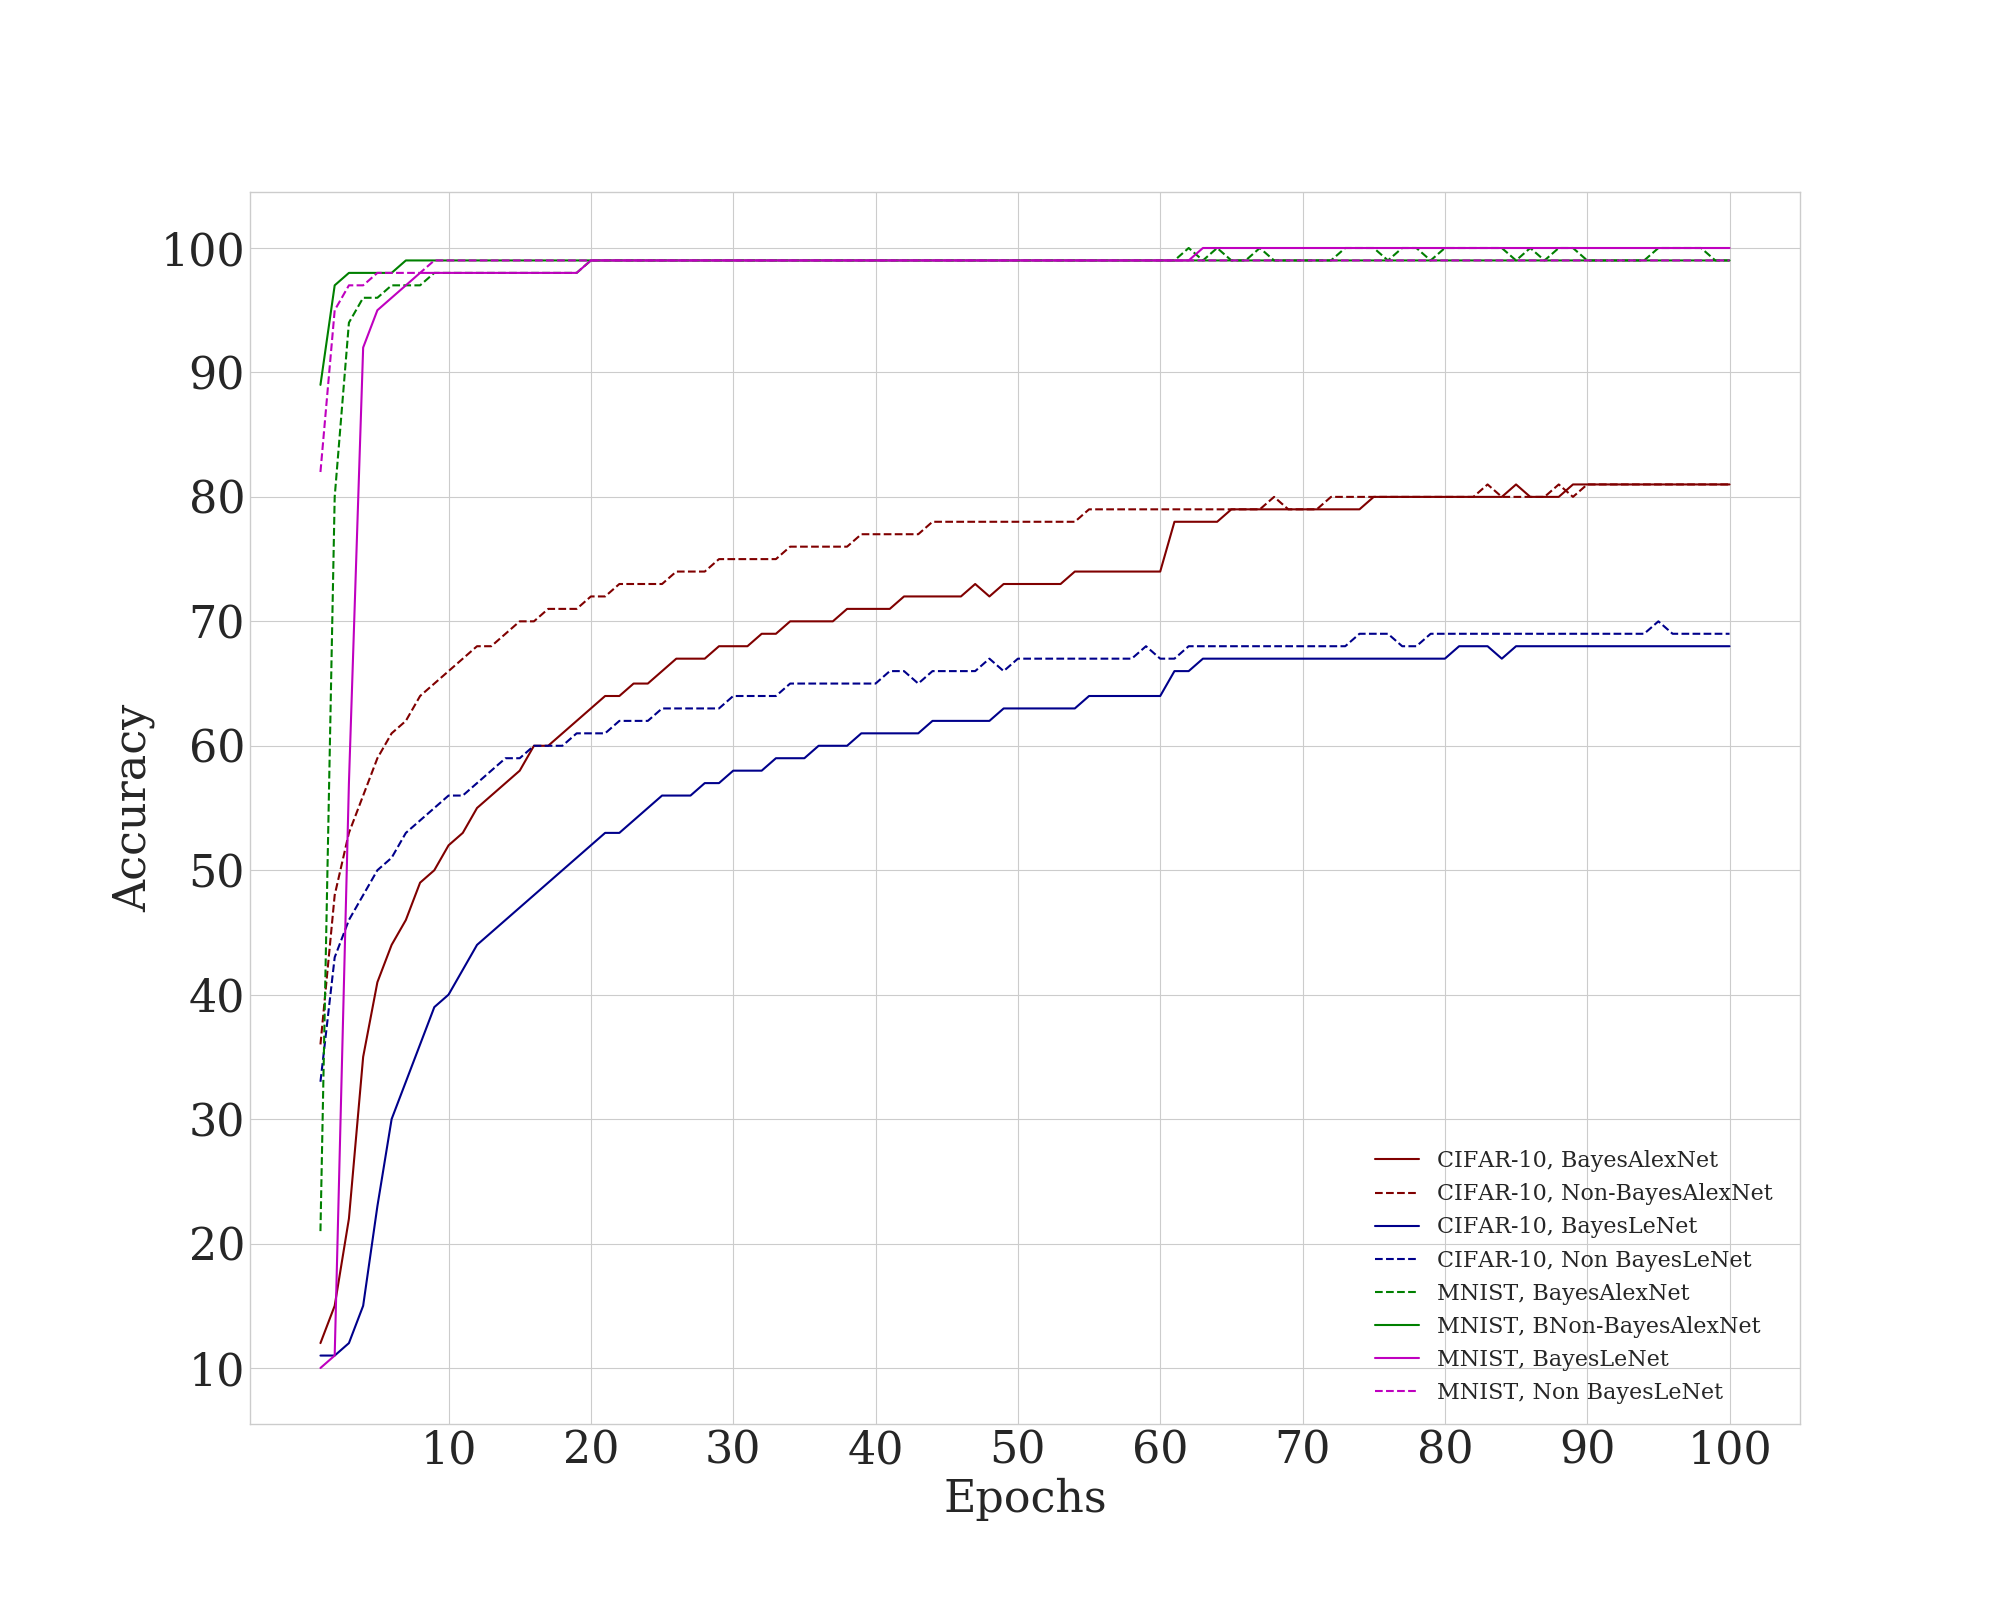
\includegraphics[width=\linewidth]{Chapter5/Figs/results_mnist_CIFAR10.png}
\caption{Comparison of Validation Accuracies of Bayesian AlexNet and LeNet-5 with frequentist approach on MNIST and CIFAR-10 datasets}
\label{fig:MnistCIFAR10reesults}
\end{center}
\end{figure} 

\newline Figure \ref{fig:MnistCIFAR10reesults} shows the validation accuracies of Bayesian vs Non-Bayesian \acp{cnn}. One thing to observe is that in initial epochs, Bayesian \acp{cnn} trained by variational inference start with a low validation accuracy compared to architectures trained by frequentist inference. This must deduce from the initialization of the variational posterior probability distributions $q_{\theta}(w|\mathcal{D})$ as uniform distributions, while initial point-estimates in architectures trained by frequentist inference are randomly drawn from a standard Gaussian distribution. (For uniformity, we changed the initialization of frequentist architectures from Xavier initialization to standard Gaussian). The latter initialization method ensures the initialized weights are neither too small nor too large. In other words, the motivation of the latter initialization is to start with weights such that the activation functions do not let them begin in saturated or dead regions. This is not true in case of uniform distributions and hence, Bayesian \acp{cnn}' starting validation accuracies can be comparably low.

\pagebreak
\newline Figure \ref{fig:std_CNN} displays the convergence of the standard deviation $\sigma$ of the variational posterior probability distribution $q_{\theta}(w|\mathcal{D})$ of a random model parameter over epochs. As aforementioned, all prior probability distributions $p(w)$ are initialized as uniform distributions. The variational posterior probability distributions $q_{\theta}(w|\mathcal{D})$ are approximated as Gaussian distributions which become more confident as more data is processed - observable by the decreasing standard deviation over epochs in Figure \ref{fig:std_CNN}. Although the validation accuracy for MNIST on Bayesian LeNet-5 has already reached 99\%, we can still see a fairly steep decrease in the parameter's standard deviation. In Figure \ref{fig:distribution}, we plot the actual Gaussian variational posterior probability distributions $q_{\theta}(w|\mathcal{D})$ of a random parameter of LeNet-5 trained on CIFAR-10 at some epochs.
%
\begin{figure}[H] 
\begin{center}
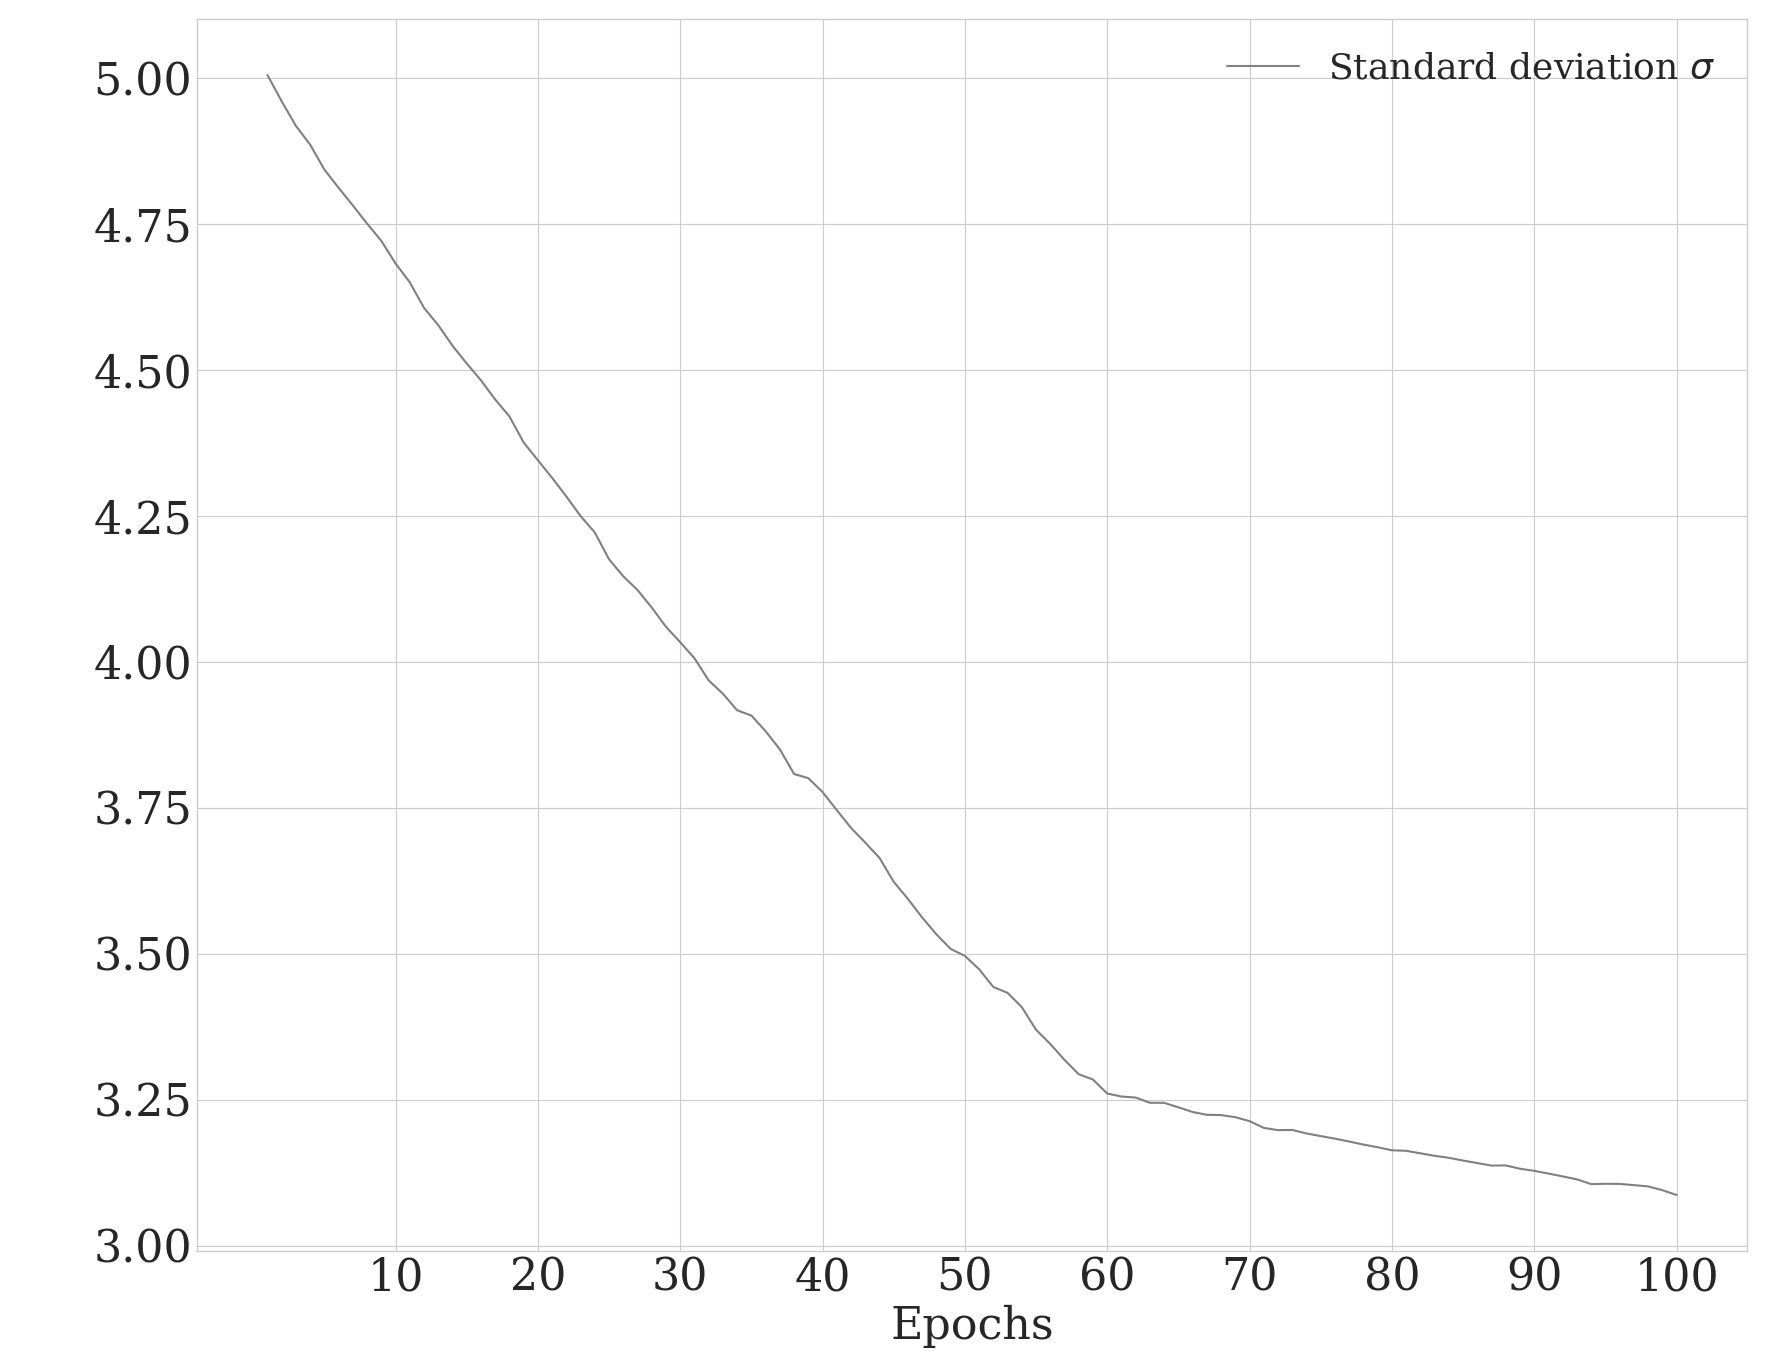
\includegraphics[width=\linewidth]{Chapter5/Figs/std_CNN.png}
\caption{Convergence of the standard deviation of the Gaussian variational posterior probability distribution $q_{\theta}(w|\mathcal{D})$ of a random model parameter at epochs 1, 5, 20, 50, and 100. MNIST is trained on Bayesian LeNet-5.}
\label{fig:std_CNN}
\end{center}
\end{figure} 
%

\begin{figure}[H] 
\begin{center}
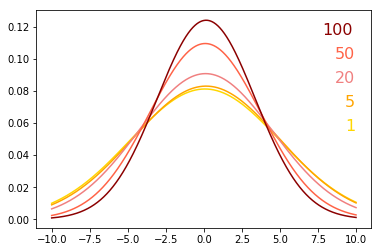
\includegraphics[width=\linewidth]{Chapter5/Figs/distribution.png}
\caption{Convergence of the Gaussian variational posterior probability distribution $q_{\theta}(w|\mathcal{D})$ of a random model parameter at epochs 1, 5, 20, 50, and 100. CIFAR-10 is trained on Bayesian LeNet-5.}
\label{fig:distribution}
\end{center}
\end{figure} 

\newline Figure \ref{fig:distribution} displays the convergence of the Gaussian variational probability distribution of a weight taken randomly from the first layer of LeNet-5 architecture. The architecture is trained on CIFAR-10 dataset with uniform initialization. 



\section{Case Study 2: Large Dataset (CIFAR-100)}
\subsection{Dataset}

\subsubsection{CIFAR-100}
This dataset is similar to the CIFAR-10 and is a labelled subset of the 80 million tiny images dataset \cite{Torralba:2008:MTI:1444381.1444403}. The dataset has 100 classes containing 600 images each. There are 500 training images and 100 validation images per class. The images are coloured with a resolution of 32 by 32 pixels.

\subsection{Results}

\begin{table}[H]
\tiny
    \centering
    \renewcommand{\arraystretch}{1.5}
    \resizebox{\linewidth}{!}{
    \begin{tabular}{ l  c  c  } 
     \hline
      \empty & CIFAR-100  \\ [0.75ex]
     \hline
     Bayesian AlexNet (with VI)  & 36  \\
     
     Frequentist AlexNet & 38  \\

     Bayesian LeNet-5 (with VI) &  31  \\
     
     Frequentist LeNet-5  & 33  \\
     \hline \\
    \end{tabular}}
    \renewcommand{\arraystretch}{1.5}
    \caption{Comparison of validation accuracies (in percentage) for different architectures with variational inference (VI), frequentist inference and Dropout as a Bayesian approximation as proposed by Gal and Ghahramani \cite{gal2015bayesian} for MNIST, CIFAR-10, and CIFAR-100.}
    \label{tab:resultsCIFAR-100}
\end{table}

In Figure \ref{fig:regularization}, we show how Bayesian networks incorporate naturally effects of regularization, exemplified on AlexNet. While an AlexNet trained by frequentist inference without any regularization overfits greatly on CIFAR-100, an AlexNet trained by Bayesian inference on CIFAR-100 does not. This is evident from the high value of training accuracy for frequentist approach with no dropout or 1 layer dropout. Bayesian CNN performs equivalently to an AlexNet trained by frequentist inference with three layers of Dropout after the first, fourth, and sixth layers in the architecture.
Another thing to note here is that the Bayesian CNN with 100 samples overfits slightly lesser compared to Bayesian CNN with 25 samples. However, a higher sampling number on a smaller dataset didn't prove useful and we stuck with 25 as the number of samples for all other experiments.


\begin{figure}[H] 
\begin{center}
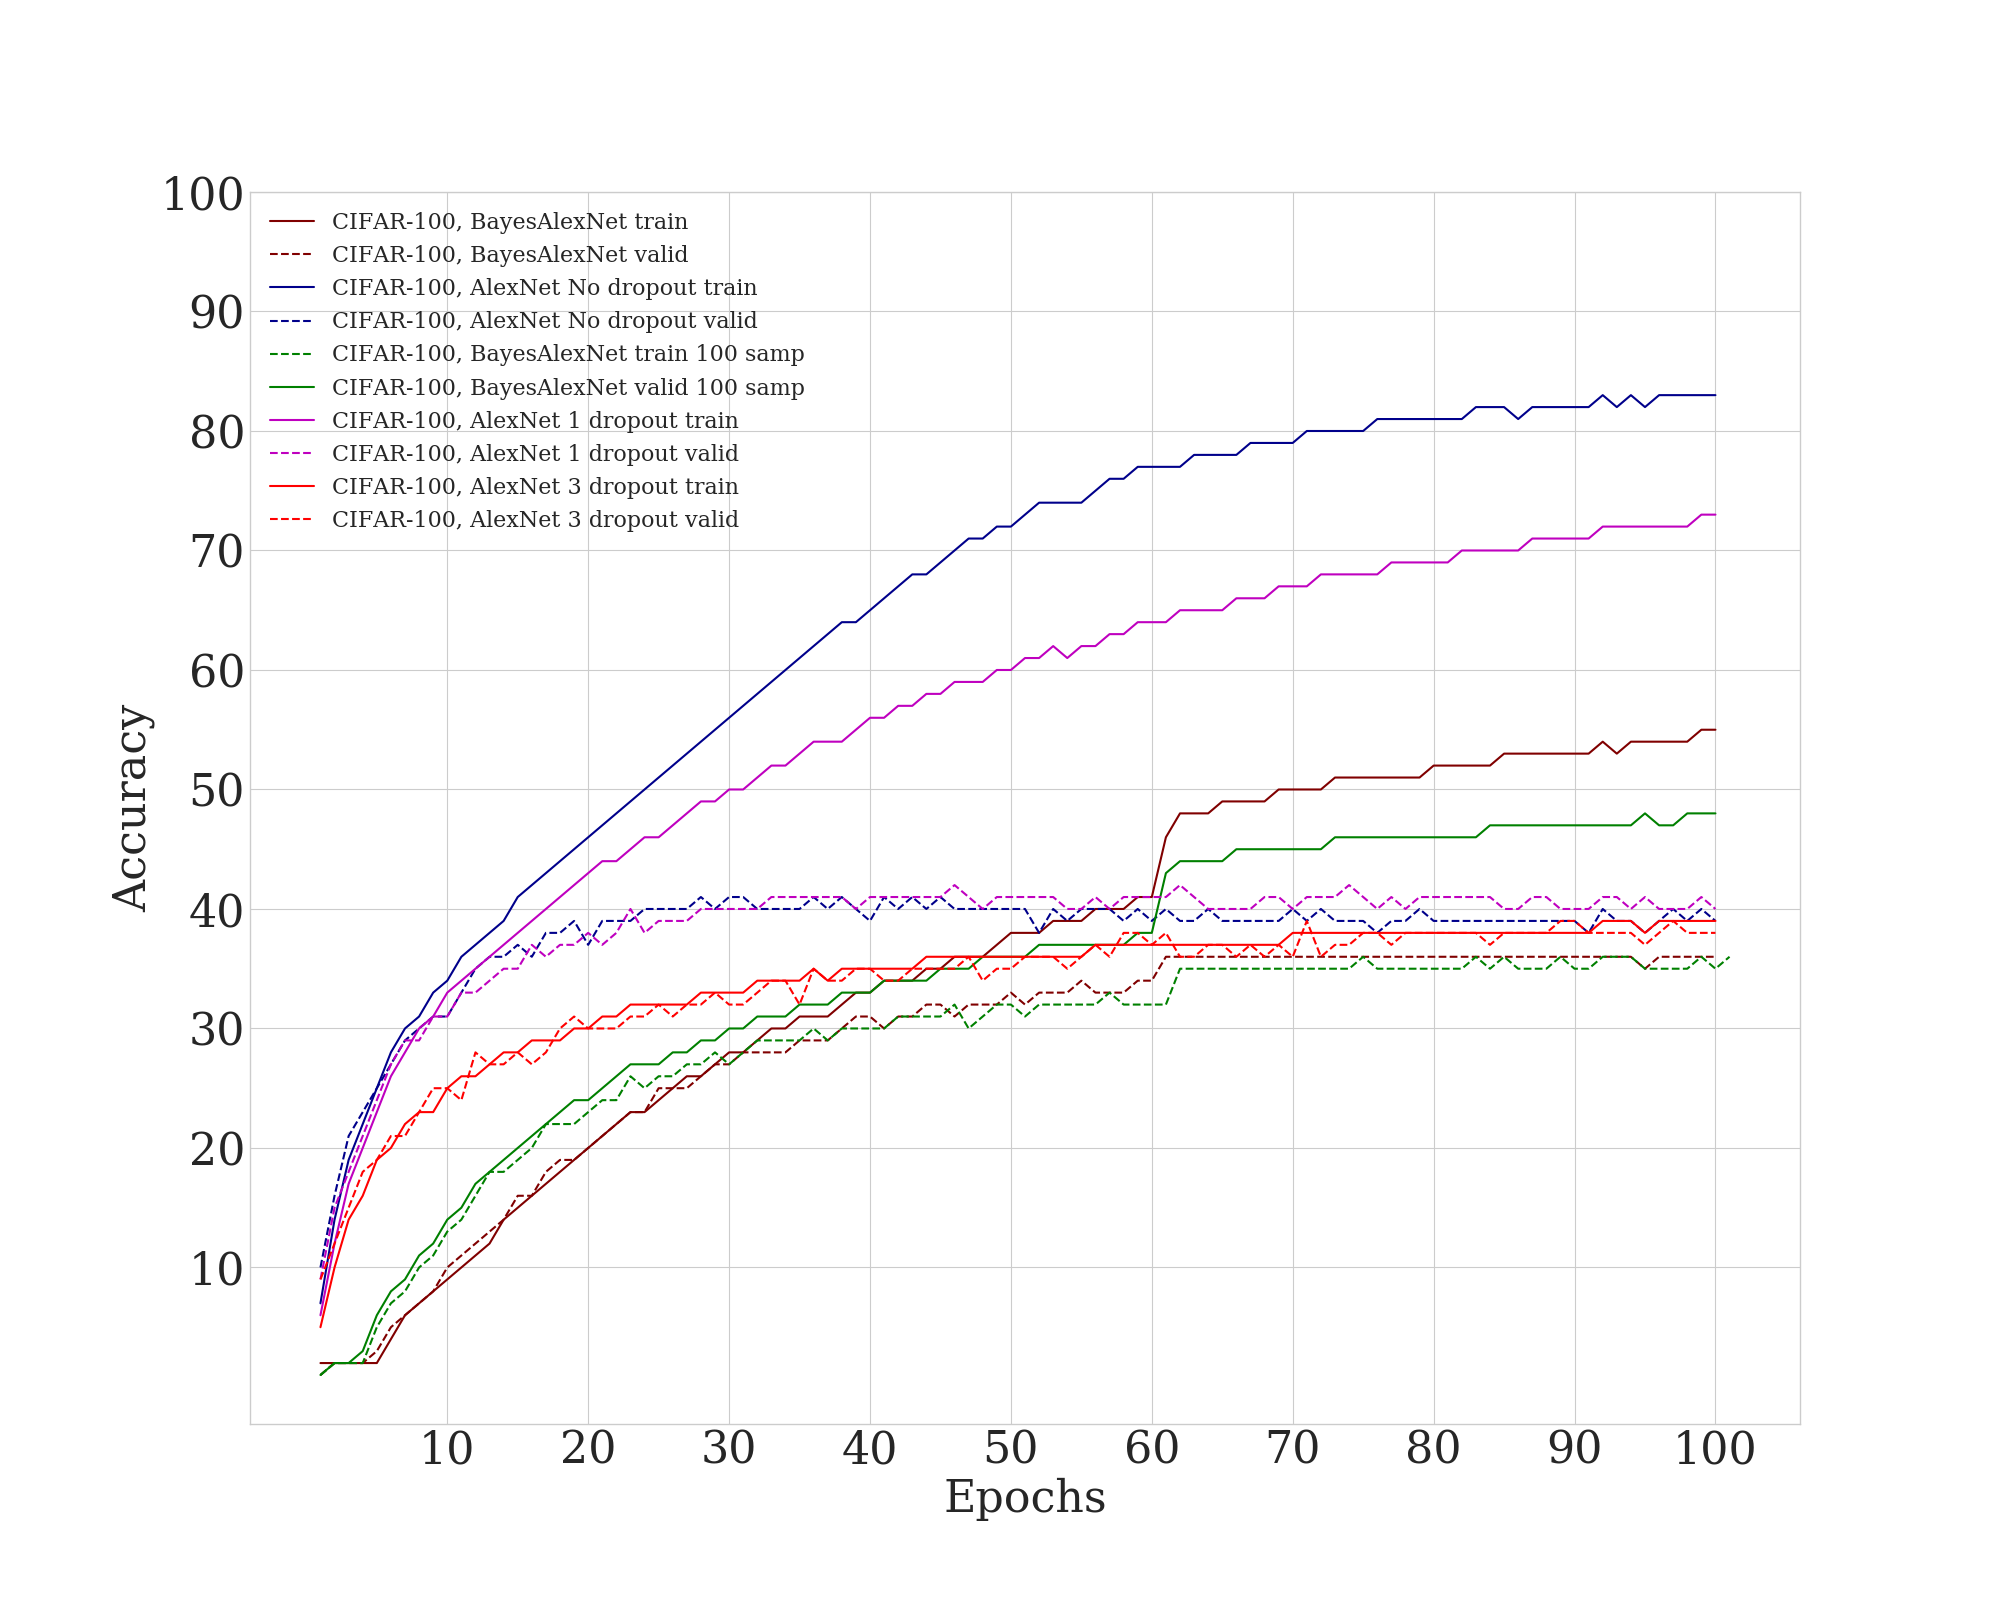
\includegraphics[width=\linewidth]{Chapter5/Figs/results_train_test_cifar100.png}
\caption{Comparison of Training and Validation Accuracies of Bayesian AlexNet and LeNet-5 with frequentist approach with and without dropouts on CIFAR-100 datasets}
\label{fig:regularization}
\end{center}
\end{figure} 

Table \ref{tab:tableCIFAR100} shows a comparison of the training and validation accuracies for AlexNet with Bayesian approach and frequentist approach. The low gap between the training and validation accuracies shows the robustness of Bayesian approach towards overfitting and shows how Bayesian approach without being regularized overfits lesser as compared to frequentist architecture with no or one dropout layer. The results are comparable with AlexNet architecture with 3 dropout layers.


\begin{table}[H]
\tiny
    \centering
    \renewcommand{\arraystretch}{1.5}
    \resizebox{\linewidth}{!}{
    \begin{tabular}{ l  c  c  c  c } 
     \hline
      \empty & Training Accuracy & Validation Accuracy   \\ [0.75ex]
     \hline
     Frequentist AlexNet (No dropout) & 83 & 38   \\
     
     Frequentist AlexNet (1 dropout layer) & 72 & 40   \\
     
      Frequentist AlexNet (3 dropout layer) & 39 & 38   \\
     \hdashline
     Bayesian AlexNet (25 num of samples) & 54 & 37   \\
     
     Bayesian AlexNet (100 num of samples) & 48 & 37   \\
     \hline \\
    \end{tabular}}
    \renewcommand{\arraystretch}{1.5}
    \caption{Comparison of training and validation accuracies (in percentage) for AlexNet architecture with variational inference (VI) and frequentist inference for CIFAR-100.}
    \label{tab:tableCIFAR100}
\end{table}

\section{Uncertainity Estimation}

\newline Finally, Table \ref{tab:uncertainty} compares the means of aleatoric and epistemic uncertainties for a Bayesian LeNet-5 with variational inference on MNIST and CIFAR-10. The aleatoric uncertainty of CIFAR-10 is about twenty times as large as that of MNIST. Considering that the aleatoric uncertainty measures the irreducible variability and depends on the predicted values, a larger aleatoric uncertainty for CIFAR-10 can be directly deduced from its lower validation accuracy and may be further due to the smaller number of training examples. The epistemic uncertainty of CIFAR-10 is about fifteen times larger than that of MNIST, which we anticipated since epistemic uncertainty decreases proportionally to validation accuracy. 
\begin{table}[H]
\tiny
    \centering
    \renewcommand{\arraystretch}{1.5}
    \resizebox{\linewidth}{!}{
    \begin{tabular}{ l  c  c  c  } 
     \hline
      \empty & Aleatoric uncertainty &  Epistemic uncertainty  \\ [0.75ex]
     \hline
     Bayesian LeNet-5 (MNIST) & 0.0096 & 0.0026   \\
     
     Bayesian LeNet-5 (CIFAR-10) & 0.1920 & 0.0404   \\
     \hline \\
    \end{tabular}} 
    \renewcommand{\arraystretch}{1.5}
    \caption{Aleatoric and epistemic uncertainty for Bayesian LeNet-5 calculated for MNIST and CIFAR-10, computed as proposed by Kwon et al. \cite{kwon2018uncertainty}.}
    \label{tab:uncertainty}
\end{table}

\section{Model Pruning}

\subsubsection{Halving the Number of Filters}

For every parameter for a frequentist inference network, Bayesian \acp{cnn} has two parameters ($\mu$, $\sigma$). Halving the number of parameters of Bayesian AlexNet ensures the number of parameters of it is comparable with a frequentist inference network. The number of filters of ALexNet is halved and a new architecture called AlexNetHalf is defined in Figure 5.4. 

\begin{table}[h!]
    \centering
    \renewcommand{\arraystretch}{2}
    \begin{tabular}{c c c c c c} 
 \hline
 layer type & width & stride & padding & input shape & nonlinearity \\ [0.5ex] 
 \hline
 convolution ($11\times11$) & 32 & 4 & 5 & $M\times3\times32\times32$ & Softplus \\ 
 
 max-pooling ($2\times2$) & \empty & 2 & 0 & $M\times32\times32\times32$ & \empty \\
 
 convolution ($5\times5$) & 96 & 1 & 2 & $M\times32\times15\times15$ & Softplus \\
 
 max-pooling ($2\times2$) & \empty & 2 & 0 & $M\times96\times15\times15$ & \empty \\
 
 convolution ($3\times3$) & 192 & 1 & 1 & $M\times96\times7\times7$ & Softplus \\
 
 convolution ($3\times3$) & 128 & 1 & 1 & $M\times192\times7\times7$ & Softplus \\
 
 convolution ($3\times3$) & 64 & 1 & 1 & $M\times128\times7\times7$ & Softplus \\
 
 max-pooling ($2\times2$) & \empty & 2 & 0 & $M\times64\times7\times7$ & \empty \\
 
 fully-connected & 64 & \empty & \empty & $M\times64$ & \empty \\ [1ex] 
 \hline
\end{tabular}
\renewcommand{\arraystretch}{1.5}
\label{tab:AlexNetHalfArchitecture}
\caption{AlexNetHalf with number of filters halved compared to the original architecture.}
\end{table}


The AlexNetHalf architecture was trained and validated on the MNIST, CIFAR10 and CIFAR100 dataset and the results are shown in Table \ref{tab:resultsAlexNetHalf}. The accuracy of pruned AlexNet with only half the number of filters compared to the normal architecture shows an accuracy gain of 6 per cent in case of CIFAR10 and equivalent performance for MNIST and CIFAR100 datasets. A lesser number of filters learn the most important features which proved better at inter-class classification could be one of the explanations for the rise in accuracy. However, upon visualization of the filters, no distinct clarification can be made to prove the previous statement. \\ 
Another possible explanation could be the model is generalizing better after the reduction in the number of filters ensuring the model is not overfitting and validation accuracy is comparatively higher. CIFAR-100 higher validation accuracy on ALexNetHalf and a lower training accuracy than Bayesian AlexNet proves the theory. Using a lesser number of filters further enhances the regularization effect and makes the model more robust against overfitting. Similar results have been achieved by Narang \cite{DBLP:journals/corr/NarangDSE17} in his work where a pruned model achieved better accuracy compared to the original architecture in a speech recognition task. Suppressing or removing the weights that have lesser or no contribution to the prediction makes the model rely its prediction on the most prominent and unique features and hence improves the prediction accuracy.

\begin{table}[H]
\tiny
    \centering
    \renewcommand{\arraystretch}{1.5}
    \resizebox{\linewidth}{!}{
    \begin{tabular}{ l  c  c  c  c } 
     \hline
      \empty & MNIST & CIFAR-10 & CIFAR-100 \\ [0.75ex]
     \hline
     Bayesian AlexNet (with VI) & 99 & 73 & 36 \\
     
     Frequentist AlexNet & 99 & 73 & 38  \\
     
     Bayesian AlexNetHalf (with VI) & 99 & 79 & 38 \\
     
     \hline \\
    \end{tabular}}
    \renewcommand{\arraystretch}{1.5}
    \caption{Comparison of validation accuracies (in percentage) for AlexNet with variational inference (VI), AlexNet with frequentist inference and AlexNet with half number of filters halved for MNIST, CIFAR-10 and CIFAR-100 datasets.}
    \label{tab:resultsAlexNetHalf}
\end{table}

\subsubsection{Applying L1 Norm}


L1 norm induces sparsity in the trained model parameters and sets some values to zero. We trained a model to some epochs (number of epochs differs across datasets as we applied early stopping when validation accuracy remains unchanged for 5 epochs). We removed the zero-valued parameters of the learned weights and keep the non-zero parameters for a trained Bayesian AlexNet on MNIST and CIFAR-10 datasets. We pruned the model to make the number of parameters in a Bayesian Network comparable to the number of parameters in the point-estimate architecture. \\ Table \ref{tab:resultsL1Norm} shows the comparison of validation accuracies of the applied L1 Norm AlexNet Bayesian architecture with Bayesian AlexNet architecture and with AlexNet frequentist architecture. We got comparable results on MNIST and CIFAR10 with the experiments and the results are shown in Table \ref{tab:resultsL1Norm}

\begin{table}[H]
\tiny
    \centering
    \renewcommand{\arraystretch}{1.5}
    \resizebox{\linewidth}{!}{
    \begin{tabular}{ l  c  c  c  } 
     \hline
      \empty & MNIST & CIFAR-10  \\ [0.75ex]
     \hline
     Bayesian AlexNet (with VI) & 99 & 73  \\
     
     Frequentist AlexNet & 99 & 73   \\
     
     Bayesian AlexNet with L1 Norm (with VI) & 99 & 71  \\
     
     \hline \\
    \end{tabular}}
    \renewcommand{\arraystretch}{1.5}
    \caption{Comparison of validation accuracies (in percentage) for AlexNet with variational inference (VI), AlexNet with frequentist inference and BayesianAlexNet with L1 norm applied for MNIST and CIFAR-10 datasets.}
    \label{tab:resultsL1Norm}
\end{table}

One thing to note here is that the numbers of parameters of Bayesian Network after applying L1 norm is not necessarily equal to the number of parameters in the frequentist AlexNet architecture. It depends on the data size and the number of classes. However, the number of parameters in the case of MNIST and CIFAR-10 are pretty comparable and there is not much reduction in the accuracy either. Also, the early stopping was applied when there is no change in the validation accuracy for 5 epochs and the model was saved and later pruned with the application of L1 norm.

\section{Training Time}

Training time of a Bayesian \acp{cnn} is twice of a frequentist network with similar architecture when the number of samples is equal to one. In general, the training time of a Bayesian \acp{cnn}, $T$ is defined as:
\begin{align}
T = 2 * number\_of\_samples * t
\end{align}
where $t$ is the training time of a frequentist network. 
The factor of 2 is present due to the double learnable parameters in a Bayesian CNN network i.e. mean and variance for every single point estimate weight in the frequentist network.

However, there is no difference in the inference time for both the networks. 


\ifpdf
    \graphicspath{{Chapter2/Figs/Raster/}{Chapter2/Figs/PDF/}{Chapter2/Figs/}}
\else
    \graphicspath{{Chapter2/Figs/Vector/}{Chapter2/Figs/}}
\fi



\chapter{Applications}


\section{BayesCNN for Image Classification}
And now I begin my third chapter here \dots

And now to cite some more people~\citet{Rea85,Ancey1996}

\section{BayesCNN for Image Super Resolution}

The task referred as Super Resolution is the recovery of a High Resolution image from a given Low Resolution image. It is applicable to many areas like medical imaging \citet{10.1007/978-3-642-40760-4_2}, face recognition \citet{1203152} and so on.

There are many ways to do a single image super resolution and a detailed benchmarks of the methods is provided by Yang \citet{Yang2014SingleImageSA}. Following are the major ways to do a single image super resolution:\\
Prediction Models. SISR algorithms in this category generate HR images
from LR inputs through a predefined mathematical formula without training
data. Interpolation-based methods (bilinear, bicubic, and Lanczos) generate HR pixel intensities by weighted averaging neighboring LR pixel values. Since interpolated intensities are locally similar to neighboring pixels, these algorithms generate good smooth regions but insufficient large gradients along edges and at high-frequency regions. The IP method [16] exploits a predefined downsampling model from a HR image to a LR image. Given an initial HR image, this method iteratively generates a LR image through the predefined downsampling model and compensates the difference map in LR back to the HR image. Since a generated HR image is designed to best match the LR input image under the linear downsampling model, the contrast along edges is better enhanced than the results generated by bicubic interpolation.\\

Edge Based Methods. Edges are important primitive image structures that
play a prime role in visual perception. Several SISR algorithms have been proposed to learn priors from edge features for reconstructing HR images. Various edge features have been proposed such as the depth and width of an edge [8] or the parameter of a gradient profile [30]. Since the priors are primarily learned from edges, the reconstructed HR images have high-quality edges with proper sharpness and limited artifacts. However, edge priors are less effective for modeling other high-frequency structures such as textures.\\

Patch Based Methods. Given a set of paired LR and HR training images,
patches can be cropped from the training images to learn mapping functions.]. In addition to equally averaging overlapped patches, several methods for blending overlapped pixels have been proposed including weighted averaging [11,44], Markov Random Fields [10], and Conditional Random Fields [38].



The global \ac{SR} problem assumes \ac{LR} data to be a low-pass filtered (blurred), downsampled and noisy version of \ac{HR} data. It is a highly ill-posed problem, due to the loss of high-frequency information that occurs during the non-invertible low-pass filtering and subsampling operations. Furthermore, the SR operation is effectively a one-to-many mapping from \ac{LR} to \ac{HR} space which can have multiple solutions, of which determining the correct solution is non-trivial. A key assumption that underlies many \ac{SR} techniques is that much of the high-frequency data is redundant and thus can be accurately reconstructed from low frequency components. \ac{SR} is therefore an inference problem, and thus relies on our model of the statistics of images in question.


\subsection{Our Approach}

We build our work upon \citet{DBLP:journals/corr/ShiCHTABRW16} work that shows that performing Super Resolution work in High Resolution space is not the optimal solution and it adds the computation complexity. We used a Bayesian Convolutional Neural Network to extract features in the Low Resolution space. We use an efficient sub-pixel convolution layer, as proposed by \citet{DBLP:journals/corr/ShiCHTABRW16}, which learns an array of upscaling filters to upscale the final Low Resolution feature maps into the High Resolution output. This replaces the handcrafted bicubic filter in the Super Resolution pipeline with more complex upscaling filters specifically trained for each feature map, and also reduces the computational complexity of the overall Super Resolution operation.

\begin{figure*}[htbp]
\begin{center}
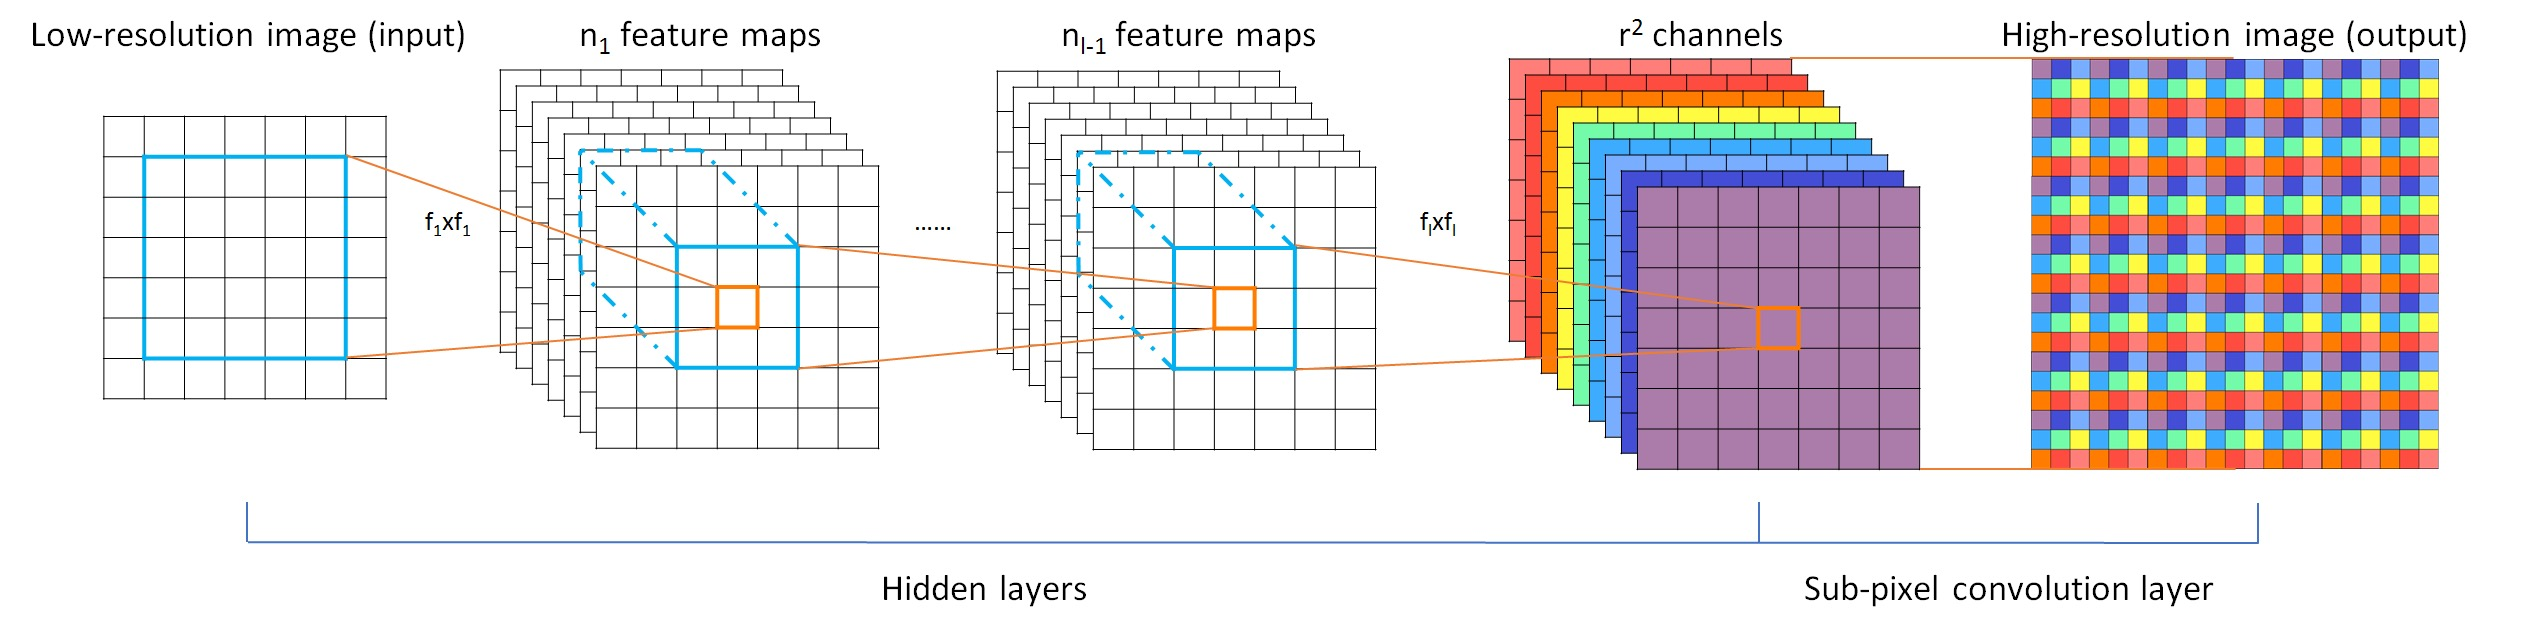
\includegraphics[width=1.0\linewidth]{Chapter6/Figs/networkstructure.jpg}
\caption{The proposed efficient sub-pixel convolutional neural network (ESPCN), with two convolution layers for feature maps extraction, and a sub-pixel convolution layer that aggregates the feature maps from \ac{LR} space and builds the \ac{SR} image in a single step.}
\label{fig:networkstructure}
\end{center}
\end{figure*}

\subsubsection{Empirical Analysis}



\section{BayesCNN for Generative Adversarial Networks}

\section{Introduction}
Generative Adversarial Networks (GANs) \cite{goodfellow2014generative} can be used for two major tasks: to learn good feature representations by using the generator and discriminator networks as feature extractors, and to generate natural images. The learned feature representation or generated images can reduce the number of images substantially for a computer vision supervised task. However GANs were quite unstable to train in the past and that is why we base our work on the stable GAN architecture namely Deep Convolutional GANs (DCGAN) \cite{DBLP:journals/corr/RadfordMC15}. We use the trained Bayesian discriminators for image classification tasks, showing competitive performance with the normal DCGAN architecture.

\section{Our approach}
\section{Empirical Analysis}




    
\fbox{
    \parbox{\textwidth}
    {
        Architecture guidelines for stable Deep Convolutional GANs
        \begin{itemize}
            \item Replace any pooling layers with strided convolutions (discriminator) and fractional-strided convolutions (generator).
            \item Use batchnorm in both the generator and the discriminator.
            \item Remove fully connected hidden layers for deeper architectures.
            \item Use ReLU activation in generator for all layers except for the output, which uses Tanh.
            \item Use LeakyReLU activation in the discriminator for all layers.
        \end{itemize}
    }
}

\chapter{Conclusion and Outlook}

We propose Bayesian \acp{cnn} utilizing \textit{Bayes by Backprop} as a reliable, variational inference method for \acp{cnn} which has not been studied to-date, and estimate the models' aleatoric and epistemic uncertainties.
\newline There has been previous work by Gal and Ghahramani \cite{gal2015bayesian} who utilized the various outputs of a Dropout function to define a distribution, and concluded that one can then speak of a Bayesian \ac{cnn}. This approach finds, perhaps also due its ease, a large confirming audience. However, we argue against this approach, and claim deficiencies. Specifically, in Gal's and Ghahramani's \cite{gal2015bayesian} approach, no prior probability distributions $p(w)$ are placed on the \ac{cnn}'s parameters. But, these are a substantial part of a Bayesian interpretation for the simple reason that Bayes' theorem includes them. Thus we argue, starting with prior probability distributions $p(w)$ is essential in Bayesian methods. In comparison, we place prior probability distributions over all model parameters, and update them according to Bayes' theorem with variational inference, precisely \textit{Bayes by Backprop}. We show that these neural networks achieve state-of-the-art results as those achieved by the same network architectures trained by frequentist inference. Furthermore, we examine how aleatoric and epistemic uncertainties can be computed for our proposed method and show the natural regularization effect of Bayesian methods.
\newline As an add-on method to further enhance the stability of the optimization, \textit{posterior sharpening} \cite{fortunato2017bayesian} could be applied to Bayesian \acp{cnn} in future work. There, the variational posterior distribution $q_{\theta}(w|\mathcal{D})$ is conditioned on the training data of a batch $\mathcal{D}^{(i)}$. We can see $q_{\theta}(w|\mathcal{D}^{(i)})$ as a proposal distribution, or \textit{hyper-prior} when we rethink it as a hierarchical model, to improve the gradient estimates of the intractable likelihood function $p(\mathcal{D}|w)$.
%



% ********************************** Back Matter *******************************
% Backmatter should be commented out, if you are using appendices after References
%\backmatter

% ********************************** Bibliography ******************************
\begin{spacing}{0.9}

% To use the conventional natbib style referencing
% Bibliography style previews: http://nodonn.tipido.net/bibstyle.php
% Reference styles: http://sites.stat.psu.edu/~surajit/present/bib.htm

\bibliographystyle{apalike}
%\bibliographystyle{unsrt} % Use for unsorted references  
\bibliographystyle{plainnat} % use this to have URLs listed in References
\cleardoublepage
\bibliography{References/references} % Path to your References.bib file


% If you would like to use BibLaTeX for your references, pass `custombib' as
% an option in the document class. The location of 'reference.bib' should be
% specified in the preamble.tex file in the custombib section.
% Comment out the lines related to natbib above and uncomment the following line.

%\printbibliography[heading=bibintoc, title={References}]


\end{spacing}

% ********************************** Appendices ********************************

\begin{appendices} % Using appendices environment for more functunality

%!TEX root = ../thesis.tex
% ******************************* Thesis Appendix A ****************************
\chapter{Experiment Specifications} 

\section*{Bayesian Settings}

\subsection{Image Recognition}

\begin{table}[H]
    \centering
    \renewcommand{\arraystretch}{2}
    \begin{tabular}[c]{c | c} 
     \hline
     variable & value \\ [0.5ex] 
     \hline
     learning rate &  0.001\\ 
     
     epochs & 100 \\
     
     batch size & 256 \\
     
     sample size & 10-25 \\
     
     loss & cross-entropy \\
     
     $(\alpha \mu^2)_{init}$ of approximate posterior $q_{\theta}(w|\mathcal{D})$ & -10 \\
     
     optimizer & Adam \cite{kingma2014adam} \\
     
     $\lambda$ in $\ell$-2 normalisation & 0.0005 \\
    
     $\beta_i$ & $\frac{2^{M-i}}{2^M-1}$ \cite{blundell2015weight} \\ [1ex] 
     \hline
    \end{tabular} 
    \renewcommand{\arraystretch}{2}
\end{table}

Sample size can vary from 10 to 25 as this range provided the best results. However, it can be played around with. For most of our experiments, it is either 10 or 25 unless specified otherwise. 

\subsection{Image Super Resolution}

\begin{table}[H]
    \centering
    \renewcommand{\arraystretch}{2}
    \begin{tabular}[c]{c | c} 
     \hline
     variable & value \\ [0.5ex] 
     \hline
     learning rate &  0.01\\ 
     
     epochs & 200 \\
     
     batch size & 64 \\
     
     upscale factor & 3 \\
     
     loss & Mean Squared Error \\
     
     seed & 123 \\
     
     $(\alpha \mu^2)_{init}$ of approximate posterior $q_{\theta}(w|\mathcal{D})$ & -10 \\
     
     optimizer & Adam \cite{kingma2014adam} \\
     
     $\lambda$ in $\ell$-2 normalisation & 0.0005 \\
    
     $\beta_i$ & $\frac{2^{M-i}}{2^M-1}$ \cite{blundell2015weight} \\ [1ex] 
     \hline
    \end{tabular} 
    \renewcommand{\arraystretch}{2}
\end{table}


\subsection{Generative Adversarial Network}

\begin{table}[H]
    \centering
    \renewcommand{\arraystretch}{2}
    \begin{tabular}[c]{c | c} 
     \hline
     variable & value \\ [0.5ex] 
     \hline
     learning rate &  0.001\\ 
     
     epochs & 100 \\
     
     batch size & 64 \\
     
     image size & 64 \\
     
     latent vector (nz) & 100 \\
     
     number of generator factor (ndf) & 64 \\
     
     number of discriminator factor (ndf) & 64 \\
     
     upscale factor & 3 \\
     
     loss & Mean Squared Error \\
     
     number of channels (nc) & 3 \\
     
     $(\alpha \mu^2)_{init}$ of approximate posterior $q_{\theta}(w|\mathcal{D})$ & -10 \\
     
     optimizer & Adam \cite{kingma2014adam} \\
     
     $\lambda$ in $\ell$-2 normalisation & 0.0005 \\
    
     $\beta_i$ & $\frac{2^{M-i}}{2^M-1}$ \cite{blundell2015weight} \\ [1ex] 
     \hline
    \end{tabular} 
    \renewcommand{\arraystretch}{2}
\end{table}

\section*{Non Bayesian Settings}

\subsection{Image Recognition}

\begin{table}[H]
    \centering
    \renewcommand{\arraystretch}{2}
    \begin{tabular}[c]{c | c} 
     \hline
     variable & value \\ [0.5ex] 
     \hline
     learning rate &  0.001\\ 
     
     epochs & 100 \\
     
     batch size & 256 \\
     
     loss & cross-entropy \\
     
     initializer & Xavier \cite{glorot2010understanding} or Normal \\
     
     optimizer & Adam \cite{kingma2014adam} \\ [1ex] 
     \hline
    \end{tabular} 
    \renewcommand{\arraystretch}{2}
\end{table}

The weights were initialized with Xavier initialization \cite{glorot2010understanding} at first, but to make it consistent with the Bayesian networks where initialization was Normal initialization (mean = 0 and variance = 1), the initializer was changed to Normal initialization.

\pagebreak

\section*{Architectures}

\subsection{LeNet-5}
 
\begin{table}[H]
    \centering
    \renewcommand{\arraystretch}{2}
    \begin{tabular}{c c c c c c} 
     \hline
     layer type & width & stride & padding & input shape & nonlinearity \\ [0.5ex] 
     \hline
     convolution ($5\times5$) & 6 & 1 & 0 & $M\times1\times32\times32$ & Softplus \\ 
     
     Mmax-pooling ($2\times2$) & \empty & 2 & 0 & $M\times6\times28\times28$ & \empty \\
     
     convolution ($5\times5$) & 16 & 1 & 0 & $M\times1\times14\times14$ & Softplus \\
     
     max-pooling ($2\times2$) & \empty & 2 & 0 & $M\times16\times10\times10$ & \empty \\
    
     fully-connected & 120 & \empty & \empty & $M\times400$ & Softplus \\
     
     fully-connected & 84 & \empty & \empty & $M\times120$ & Softplus \\
     
     fully-connected & 10 & \empty & \empty & $M\times84$ & \empty \\ [1ex] 
     \hline
    \end{tabular} 
    \renewcommand{\arraystretch}{1}
    \label{tab:LeNet}
    \caption{LeNet architecture with original configurations as defined in the paper. \cite{lecun1998gradient}}
\label{tab:AlexNet}

\end{table}

\subsection{AlexNet}

\begin{table}[H]
    \centering
    \renewcommand{\arraystretch}{2}
    \begin{tabular}{c c c c c c} 
 \hline
 layer type & width & stride & padding & input shape & nonlinearity \\ [0.5ex] 
 \hline
 convolution ($11\times11$) & 64 & 4 & 5 & $M\times3\times32\times32$ & Softplus \\ 
 
 max-pooling ($2\times2$) & \empty & 2 & 0 & $M\times64\times32\times32$ & \empty \\
 
 convolution ($5\times5$) & 192 & 1 & 2 & $M\times64\times15\times15$ & Softplus \\
 
 max-pooling ($2\times2$) & \empty & 2 & 0 & $M\times192\times15\times15$ & \empty \\
 
 convolution ($3\times3$) & 384 & 1 & 1 & $M\times192\times7\times7$ & Softplus \\
 
 convolution ($3\times3$) & 256 & 1 & 1 & $M\times384\times7\times7$ & Softplus \\
 
 convolution ($3\times3$) & 128 & 1 & 1 & $M\times256\times7\times7$ & Softplus \\
 
 max-pooling ($2\times2$) & \empty & 2 & 0 & $M\times128\times7\times7$ & \empty \\
 
 fully-connected & 128 & \empty & \empty & $M\times128$ & \empty \\ [1ex] 
 \hline
\end{tabular}
\renewcommand{\arraystretch}{1}
\caption{AlexNet architecture with original configurations as defined in the paper. \cite{krizhevsky2012imagenet}}
\label{tab:AlexNet}
\end{table}


\subsection{AlexNetHalf}

\begin{table}[H]
    \centering
    \renewcommand{\arraystretch}{2}
    \begin{tabular}{c c c c c c} 
 \hline
 layer type & width & stride & padding & input shape & nonlinearity \\ [0.5ex] 
 \hline
 convolution ($11\times11$) & 32 & 4 & 5 & $M\times3\times32\times32$ & Softplus \\ 
 
 max-pooling ($2\times2$) & \empty & 2 & 0 & $M\times32\times32\times32$ & \empty \\
 
 convolution ($5\times5$) & 96 & 1 & 2 & $M\times32\times15\times15$ & Softplus \\
 
 max-pooling ($2\times2$) & \empty & 2 & 0 & $M\times96\times15\times15$ & \empty \\
 
 convolution ($3\times3$) & 192 & 1 & 1 & $M\times96\times7\times7$ & Softplus \\
 
 convolution ($3\times3$) & 128 & 1 & 1 & $M\times192\times7\times7$ & Softplus \\
 
 convolution ($3\times3$) & 64 & 1 & 1 & $M\times128\times7\times7$ & Softplus \\
 
 max-pooling ($2\times2$) & \empty & 2 & 0 & $M\times64\times7\times7$ & \empty \\
 
 fully-connected & 64 & \empty & \empty & $M\times64$ & \empty \\ [1ex] 
 \hline
\end{tabular}
\renewcommand{\arraystretch}{1.5}
\label{tab:AlexNetHalfArchitecture}
\caption{AlexNetHalf with number of filters halved compared to the original architecture.}
\end{table}


%!TEX root = ../thesis.tex
% ******************************* Thesis Appendix B ********************************

\chapter{How to replicate results}

Install PyTorch from the official website (\url{https://pytorch.org/})

\begin{verbatim} 

git clone https://github.com/kumar-shridhar/PyTorch-BayesianCNN
pip install -r requirements.txt

\end{verbatim}
\textit{cd} into respective folder/ task to replicate (Image Recognition, Super Resolution or GAN)

\subsection{Image Recognition}

\begin{verbatim} 
python main_Bayesian.py
\end{verbatim}

to replicate the Bayesian \acp{cnn} results.

\begin{verbatim} 
python main_nonBayesian.py
\end{verbatim}

to replicate the Frequentist \acp{cnn} results.\\

\\For more details, read the README sections of the repo : \url{https://github.com/kumar-shridhar/PyTorch-BayesianCNN}




\end{appendices}

% *************************************** Index ********************************
\printthesisindex % If index is present

\end{document}
